%% PNAStmpl.tex
%% Template file to use for PNAS articles prepared in LaTeX
%% Version: Apr 14, 2008


%%%%%%%%%%%%%%%%%%%%%%%%%%%%%%
%% BASIC CLASS FILE
%% PNAStwo for two column articles is called by default.
%% Uncomment PNASone for single column articles. One column class
%% and style files are available upon request from pnas@nas.edu.
%% (uncomment means get rid of the '%' in front of the command)

%\documentclass{pnasone}
\documentclass{pnastwo}

%%%%%%%%%%%%%%%%%%%%%%%%%%%%%%
%% Changing position of text on physical page:
%% Since not all printers position
%% the printed page in the same place on the physical page,
%% you can change the position yourself here, if you need to:

% \advance\voffset -.5in % Minus dimension will raise the printed page on the
                         %  physical page; positive dimension will lower it.

%% You may set the dimension to the size that you need.

%%%%%%%%%%%%%%%%%%%%%%%%%%%%%%
%% OPTIONAL GRAPHICS STYLE FILE

%% Requires graphics style file (graphicx.sty), used for inserting
%% .eps files into LaTeX articles.
%% Note that inclusion of .eps files is for your reference only;
%% when submitting to PNAS please submit figures separately.

%% Type into the square brackets the name of the driver program
%% that you are using. If you don't know, try dvips, which is the
%% most common PC driver, or textures for the Mac. These are the options:

% [dvips], [xdvi], [dvipdf], [dvipdfm], [dvipdfmx], [pdftex], [dvipsone],
% [dviwindo], [emtex], [dviwin], [pctexps], [pctexwin], [pctexhp], [pctex32],
% [truetex], [tcidvi], [vtex], [oztex], [textures], [xetex]

%\usepackage[dvips]{graphicx}

%%%%%%%%%%%%%%%%%%%%%%%%%%%%%%
%% OPTIONAL POSTSCRIPT FONT FILES

%% PostScript font files: You may need to edit the PNASoneF.sty
%% or PNAStwoF.sty file to make the font names match those on your system.
%% Alternatively, you can leave the font style file commands commented out
%% and typeset your article using the default Computer Modern
%% fonts (recommended). If accepted, your article will be typeset
%% at PNAS using PostScript fonts.


% Choose PNASoneF for one column; PNAStwoF for two column:
%\usepackage{PNASoneF}
%\usepackage{PNAStwoF}

%%%%%%%%%%%%%%%%%%%%%%%%%%%%%%
%% ADDITIONAL OPTIONAL STYLE FILES

%% The AMS math files are commonly used to gain access to useful features
%% like extended math fonts and math commands.

\usepackage{amssymb,amsfonts,amsmath}

\usepackage{subcaption}
\graphicspath{ {paper_figures/} }


%%%%%%%%%%%%%%%%%%%%%%%%%%%%%%
%% OPTIONAL MACRO FILES
%% Insert self-defined macros here.
%% \newcommand definitions are recommended; \def definitions are supported

%\newcommand{\mfrac}[2]{\frac{\displaystyle #1}{\displaystyle #2}}
%\def\s{\sigma}

\DeclareMathOperator*{\argmin}{arg\,min}

\makeatletter
\newcommand{\customlabel}[2]{%
\protected@write \@auxout {}{\string \newlabel {#1}{{#2}{}}}}
\makeatother

%%%%%%%%%%%%%%%%%%%%%%%%%%%%%%
%% Don't type in anything in the following section:
%%%%%%%%%%%%
%% For PNAS Only:
\contributor{Submitted to Proceedings
of the National Academy of Sciences of the United States of America}
\url{www.pnas.org/cgi/doi/10.1073/pnas.0709640104}
\copyrightyear{2008}
\issuedate{Issue Date}
\volume{Volume}
\issuenumber{Issue Number}
%%%%%%%%%%%%

\begin{document}

%%%%%%%%%%%%%%%%%%%%%%%%%%%%%%


%% For titles, only capitalize the first letter
%% \title{Almost sharp fronts for the surface quasi-geostrophic equation}

\title{Unscrambling arrested development: temporal ordering and registration of cross-sectional imaging data}


%% Enter authors via the \author command.
%% Use \affil to define affiliations.
%% (Leave no spaces between author name and \affil command)

%% Note that the \thanks{} command has been disabled in favor of
%% a generic, reserved space for PNAS publication footnotes.

%% \author{<author name>
%% \affil{<number>}{<Institution>}} One number for each institution.
%% The same number should be used for authors that
%% are affiliated with the same institution, after the first time
%% only the number is needed, ie, \affil{number}{text}, \affil{number}{}
%% Then, before last author ...
%% \and
%% \author{<author name>
%% \affil{<number>}{}}

%% For example, assuming Garcia and Sonnery are both affiliated with
%% Universidad de Murcia:
%% \author{Roberta Graff\affil{1}{University of Cambridge, Cambridge,
%% United Kingdom},
%% Javier de Ruiz Garcia\affil{2}{Universidad de Murcia, Bioquimica y Biologia
%% Molecular, Murcia, Spain}, \and Franklin Sonnery\affil{2}{}}

\author{Carmeline~J.~Dsilva\affil{1}{Department of Chemical and Biological Engineering, Princeton University, Princeton, New Jersey, USA},
Bomyi~Lim\affil{1}{},
Thomas~J.~Levario\affil{2}{School of Chemical and Biomolecular Engineering, Georgia Institute of Technology, Atlanta, Georgia, USA},
Hang~Lu\affil{2}{},
Amit~Singer\affil{3}{Department of Mathematics, Princeton University, Princeton, New Jersey, USA} \affil{4}{Program in Applied and Computational Mathematics, Princeton University, Princeton, New Jersey, USA},
Stanislav~Y.~Shvartsman\affil{1}{} \affil{5}{Lewis-Sigler Institute for Integrative Genomics, Princeton University, Princeton, New Jersey, USA},
\and
Ioannis~G.~Kevrekidis\affil{1}{} \affil{4}{Program in Applied and Computational Mathematics, Princeton University, Princeton, New Jersey, USA}}

\contributor{Submitted to Proceedings of the National Academy of Sciences
of the United States of America}

%% The \maketitle command is necessary to build the title page.
\maketitle

%%%%%%%%%%%%%%%%%%%%%%%%%%%%%%%%%%%%%%%%%%%%%%%%%%%%%%%%%%%%%%%%
\begin{article}

\begin{abstract}
In studies of development, researchers are often presented with cross-sectional data, where each data point is a sample from a population fixed at a slightly different developmental time.
%
The goal is then to temporally order the data to reconstruct the developmental dynamics.
%
If each data point is a two-dimensional image, the images must first be registered before they can be temporally ordered.
%
When such data sets are large, noisy, and/or if the developmental changes are subtle, these tasks can be difficult to do by hand.
%
We present an automatic approach to register {\em and} temporally order cross-sectional data sets of images.
%
The mathematical techniques (angular synchronization for image registration, diffusion maps for temporal ordering, and
vector diffusion maps for simultaneously performing both tasks) are applicable to a wide variety of data sets and
require little {\em a priori} knowledge of the image features or the developmental dynamics.
%
We demonstrate the utility of our methods using a collection of images from a study of {\em Drosophila} embryogenesis.
\end{abstract}


%% When adding keywords, separate each term with a straight line: |
\keywords{temporal ordering | image registration}

%% Optional for entering abbreviations, separate the abbreviation from
%% its definition with a comma, separate each pair with a semicolon:
%% for example:
%% \abbreviations{SAM, self-assembled monolayer; OTS,
%% octadecyltrichlorosilane}

% \abbreviations{}

%% The first letter of the article should be drop cap: \dropcap{}
%\dropcap{I}n this article we study the evolution of ''almost-sharp'' fronts

%% Enter the text of your article beginning here and ending before
%% \begin{acknowledgements}
%% Section head commands for your reference:
%% \section{}
%% \subsection{}
%% \subsubsection{}

\dropcap{E}xperimental studies of developmental dynamics fall in two broadly defined categories: longitudinal and cross-sectional \cite{diggle2002analysis}.
%
In longitudinal studies, developmental progress is monitored over time for the same embryo.
%
In a cross-sectional study, one embryo contributes only a single snapshot of a chemical or morphological process along its developmental trajectory, and the developmental dynamics must be reconstructed from multiple snapshots of different embryos.
%
Both of these sampling schemes have their advantages and limitations, and both are extensively used by developmental biologists.
%
Here we focus on cross-sectional studies, which have a time-honored history and still present the only option for most organisms.
%
In a typical cross-sectional study, a group of developing embryos is fixed using a procedure that arrests their development and stained with chemicals that help visualize a handful of cellular processes.
%
Fixed embryos are then imaged using any given number of microscopy techniques.
%
Recent advances in large-scale physical manipulation and imaging of embryos have produced rapidly increasing volumes of cross-sectional data, in which every embryo is observed at a different geometric orientation and developmental time point.
%
Importantly, the ``age'' of any given embryo arrested in its development is not known to high accuracy.
%
In general, it is only known that a collection of embryos belongs to a certain time window.
%
In order to mine such image datasets for the developmental dynamics, snapshots of different embryos must be spatially aligned or registered to factor out the relevant symmetries (i.e., translations and rotations), and ordered in time.
%
We present a general computational framework which greatly accelerates -and can combine- both of these tasks.

Temporal ordering and registration of images is straightforward when the number of images is small and differences between them are visually apparent.
%
As an example, Figure~\ref{fig:fish} shows a caricature of fish development, combining the processes of growth and color patterning.
%
In this case, temporal ordering can be accomplished by arranging the fish by size, which uniquely correlates with the progress of development.
%
Image registration is based on obvious morphological landmarks, such as the position of head and fins.
%
On the other hand, real data poses nontrivial challenges, due to the number of images, measurement noise and variability, and the subtlety of the developmental changes.

To illustrate the issues associated with temporal ordering and registration of images, we use a data set from an imaging study of signaling protein expression in the early fruit fly embryo, one of the leading model systems for studies of developmental dynamics.
%
This dataset comprises $49$ fluorescence microscopy images of different embryos fixed during the $3^{rd}$ hour of their development.
%
\begin{figure}[t]
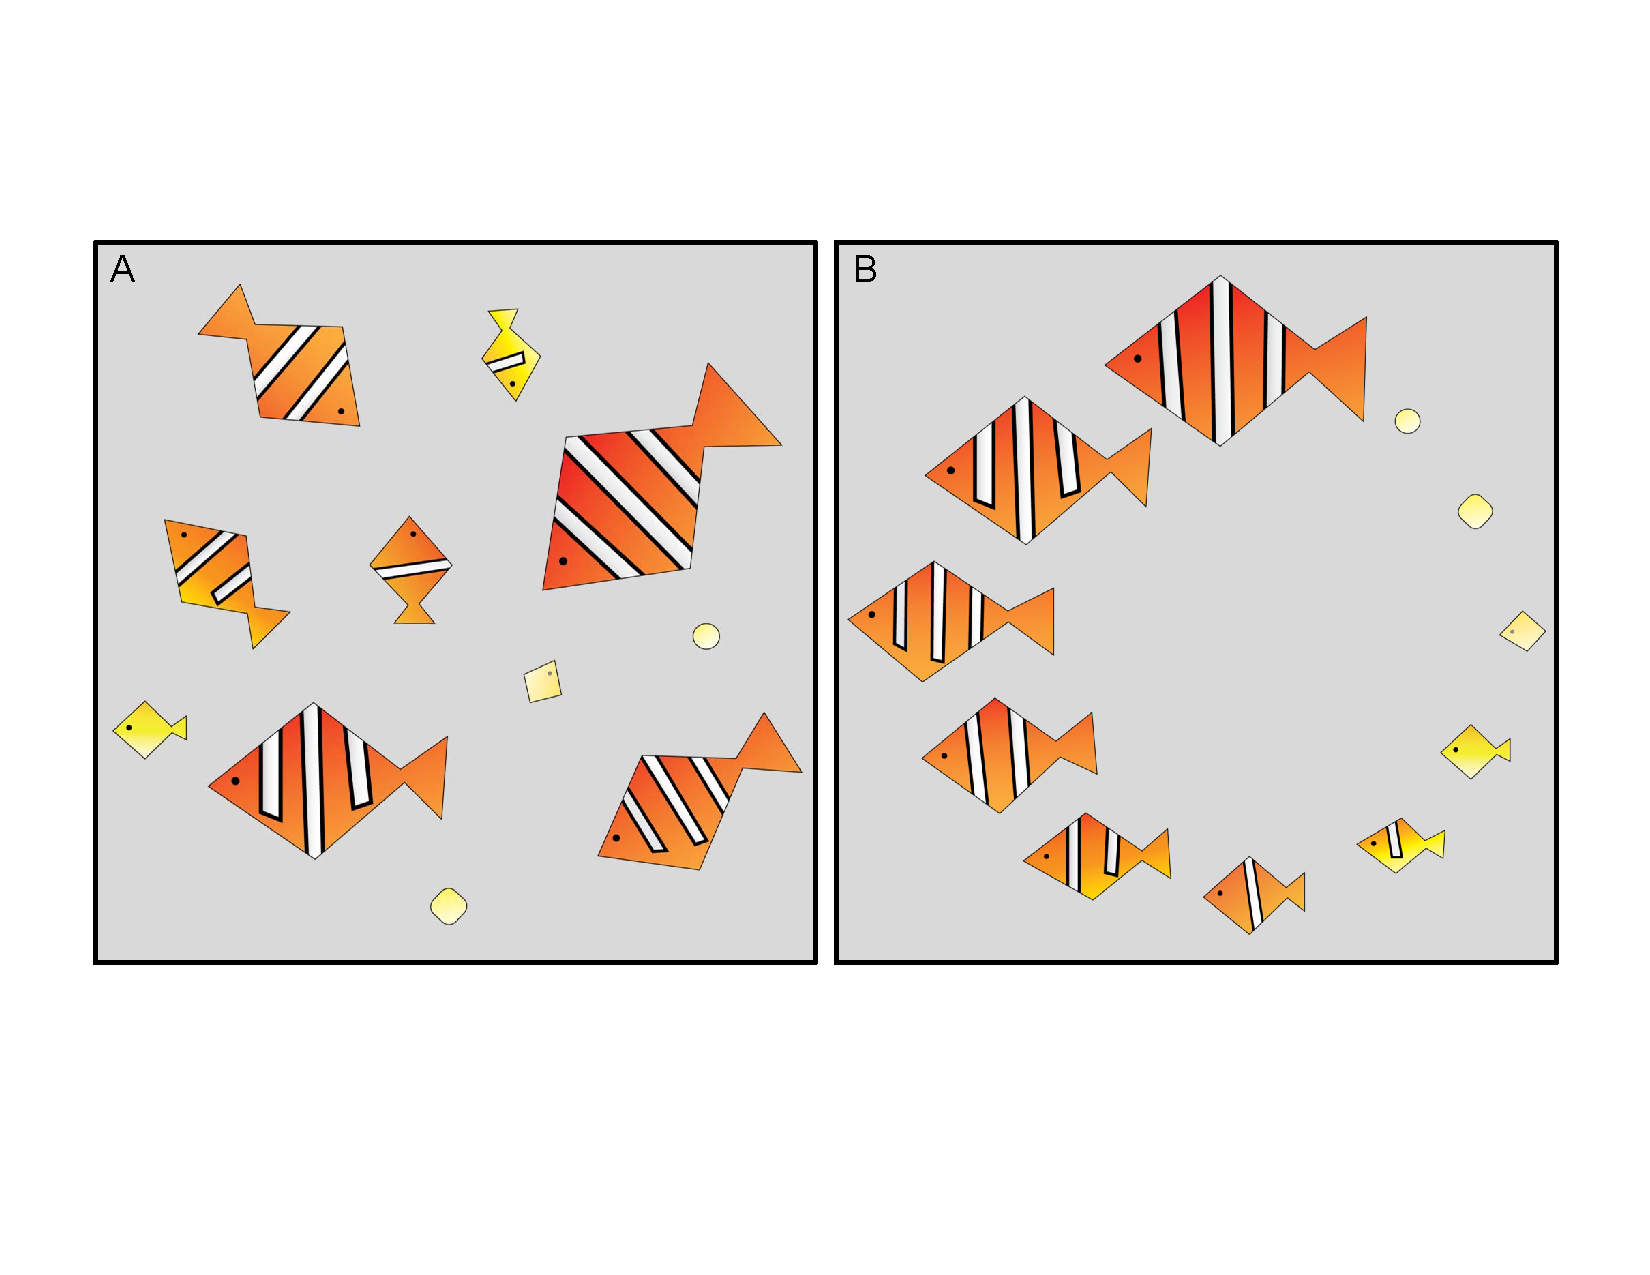
\includegraphics[width=8.4cm]{fig1}
\caption{Schematic illustration of reconstructing dynamics from cross-sectional data. (a) Fish, each in a different orientation and a different stage of development. (b) Fish, now rotationally registered and temporally ordered. For this example, the registration and ordering is easy to do ``by hand" because the data set is small and the developmental changes are easy to recognize.}
%\label{fig:fish}
\customlabel{fig:fish}{1}
\customlabel{subfig:fish_unordered}{\ref{fig:fish}a}
\customlabel{subfig:fish_ordered}{\ref{fig:fish}b}
\end{figure}
%
The fruit fly embryo is shaped like a rice grain, approximately $1/2$~mm long.
%
By end of the $2^{nd}$ hour of development, sequential divisions of a fertilized egg generate a system where $\sim 6,000$ nuclei are uniformly arranged under the common plasma membrane.
%
During the $3^{rd}$ hour, the embryo undergoes the process of cellularization, whereby membranes that enclose nuclei into different cells grow in thickness (Figure~\ref{subfig:membranes}).
%
Concurrently with these morphological changes, concentration profiles of multiple regulatory molecules form inside the embryo, subdividing it into regions that give rise to future tissues and organs \cite{lim2013kinetics}.
%
Images in Figure~\ref{subfig:images_unordered} show optical sections perpendicular to the long axis of the embryo.
%%%
%%% we have to somehow say that it is consistent
%%%
%
%%%
%%% ask if "visualize" is typical as active verb
%%%
The embryos were fixed and stained with chemicals that help visualize nuclei (shown in gray) as well as the spatial distributions of two different proteins (shown in green and red) \cite{chung2010microfluidic}.
%
Each of the images reveals a uniform arrangement of nuclei and a nonuniform distribution of the two proteins, which are involved in patterning of the dorsoventral (back-to-belly) axis of the embryo.

\begin{figure}[t]
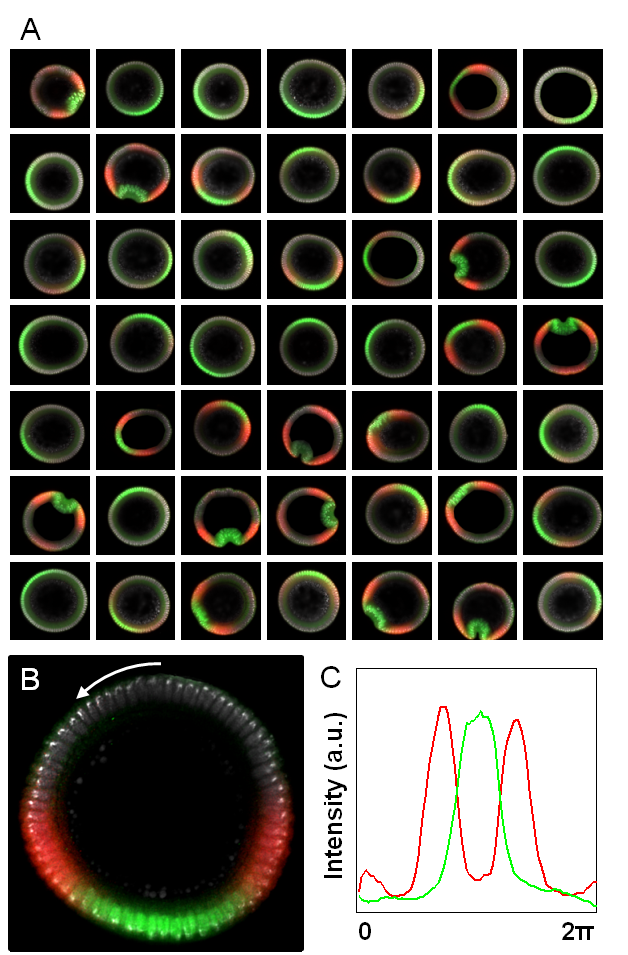
\includegraphics[width=8.4cm]{fig2}
\caption{(a) Fluorescent images of {\em Drosophila} embryos. Each embryo has been stained for Dorsal (green) and dpERK (red). (b) Selected image from data set. (c) Profile of Dorsal (green) and dpERK (red) around the circumference of the embryo in (b).}
%\label{fig:images_unordered}
\customlabel{fig:images_unordered}{2}
\customlabel{subfig:images_unordered}{\ref{fig:images_unordered}a}
\customlabel{subfig:one_image}{\ref{fig:images_unordered}b}
\customlabel{subfig:image_profiles}{\ref{fig:images_unordered}c}
\end{figure}


%%%
%%% orientation does not read good to Y below -
%%% it is the same orientation, but a different rotation around the axis
%%% how to say this ?
%%%
Each image in Figure~\ref{subfig:images_unordered} comes from a different embryo, captured at a different rotation about the long axis and at a different and unknown point in time.
%
The goal is to register these images in a globally consistent way and order them to be representative of the underlying developmental trajectory.
%
Both of these tasks can be fully automated, and even combined.
%
We will use {\em angular synchronization} \cite{singer2011angular}, a registration algorithm that is robust to noise, to align the images in a consistent way.
%
We will use {\em diffusion maps} \cite{coifman2005geometric}, a broadly applicable technique for the discovery of low-dimensional structures in high-dimensional data sets, to temporally order our data.
%
We will also show how both steps can be combined using {\em vector diffusion maps} \cite{singer2012vector}.
%
%The paper is organized as follows.
%
%First, we use a synthetic dataset, where the correct orientation and ordering of data points is known, to formalize the tasks of image registration and temporal ordering.
%
%Then, we show that both of these tasks can be effectively combined in a single step.
%
%Following this, we return to the original set of two-dimensional images and demonstrate that our approach can readily align them and order them correctly in time.
%
%We conclude by discussing the general requirements that must be satisfied for our approach to work and compare it to other approaches and ideas in cross-sectional studies of biological dynamics.

\section{Results and Discussion}

%We would like to temporally order images, such as the images shown in Figure~\ref{subfig:images_unordered}.
%
%We will use diffusion maps, a dimensionality reduction algorithm, to automatically order our data.
%
%However, this algorithm requires distances between data points.
%
%Because each image is in a different orientation, we need to first align or {\em register} the images before computing distances.
%
%Once all the images have been aligned, we can compute distances and use diffusion maps to temporally order the data.

%%%
%%%  Y to discuss with S
%%%  I think we should have the real data
%%%
%%%  also, these dynamics "are like" our dynamics
%%%
%%%   even if this is kept, one should say that this chosen because it LOOKS LIKE what we have
%%% another reason I want to have the real data is because in the discussion I want to talk about the flips
%%%

We will first demonstrate our techniques for registration and temporal ordering using a synthetic data set whose features resemble those in our imaging data set in Figure~\ref{subfig:images_unordered}.
%
This data set will allow us to illustrate the main points of the different algorithms, and will also have relatively simple dynamics which are easy to visualize.
%
We construct concentration profiles defined on a ring, and we assume that each ring is arbitrarily rotated around its center; an example is shown in Figure~\ref{subfig:1d_example}.
%
Rotation of the ring corresponds to shifting (with periodic boundary conditions) the one-dimensional concentration profile shown in the bottom of Figure~\ref{subfig:1d_example}; the symmetry group is the group of all two-dimensional proper rotations, denoted $SO(2)$.
%
Each concentration profile is a noisy Gaussian (shown in Figure~\ref{subfig:1d_intensity}), and the Gaussians increase in intensity as  a function of time.
%
We discretize the profiles into $100$ points, so our numerical data will be $100$-dimensional vectors (the corresponding symmetry group for the discretized profiles is $\mathbb{Z}_n$, the group of integers modulo $n$).
%
Figure \ref{subfig:1d_unaligned_unordered} shows the entire data set; the concentration profiles have been stacked in an array, so that each row corresponds to a single profile.
%
Because the profiles are unregistered and unordered, the underlying dynamics (a Gaussian whose amplitude grows in time) are not readily apparent.

\begin{figure}[t]
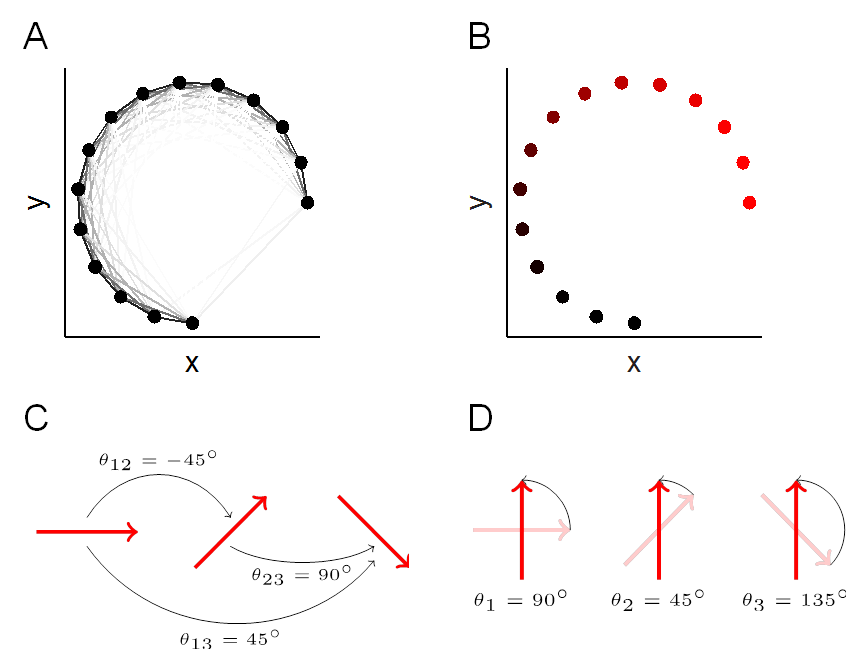
\includegraphics[width=8.4cm]{fig3}
\caption{(a) One-dimensional concentration profile on a ring (top), and the corresponding profile on a line (bottom). (b) Intensity corresponding to the profile in (a). (c) An ensemble of concentration profiles, each of the form described in (a). Each row in the array corresponds to a single profile. (d) The profiles in (c), now registered using angular synchronization. (e) The profiles in (c), now temporally ordered using diffusion maps. (f) The profiles in (c), registered and temporally ordered in a single step using vector diffusion maps.}
%\label{fig:1d_demo}
\customlabel{fig:1d_demo}{3}
\customlabel{subfig:1d_example}{\ref{fig:1d_demo}a}
\customlabel{subfig:1d_intensity}{\ref{fig:1d_demo}b}
\customlabel{subfig:1d_unaligned_unordered}{\ref{fig:1d_demo}c}
\customlabel{subfig:1d_aligned_unordered}{\ref{fig:1d_demo}d}
\customlabel{subfig:1d_aligned_ordered}{\ref{fig:1d_demo}e}
\customlabel{subfig:1d_aligned_ordered_vdm}{\ref{fig:1d_demo}f}
\end{figure}

\subsection{Angular synchronization for image registration}

We begin by registering the set of profiles using angular synchronization\cite{singer2011angular}, a technique which is robust to noise and requires no {\em a priori} knowledge of image features.
%
Angular synchronization first aligns every possible pair of data points, i.e., it computes the rotation angles
required to make each pair have the maximum possible overlap (see {\it Materials and Methods}).
%%%
%%% so I do not like the figure with the vectors - it is correct, but people have to take the
%%% function, discretize and make it a vector in their heads, and may be "one step too much"
%%%
%
An illustration is shown in Figure~\ref{subfig:synch1};
each data point is a vector, and $\theta_{ij}$ denotes the angle of rotation needed to align vectors $i$ and $j$.
%
From this large collection of pairwise alignments, the algorithm then selects a set of rotation angles $\theta_i$, one for each data point, such that differences in rotation angles $\theta_i-\theta_j$ are {\em most consistent} (in some metric) with the pairwise alignments $\theta_{ij}$.
%
Figure~\ref{subfig:synch2} shows each vector from Figure~\ref{subfig:synch1}, now rotated so that the entire set is aligned; the computed rotation angles are also indicated.
%
Note that the differences between the rotation angles assigned to each vector are consistent with the pairwise angles needed to rotate one vector to another, i.e., $\theta_i - \theta_j \approx \theta_{ij}$.
%
To compute these alignments, the task is formulated as an optimization problem, and then relaxed to an eigenproblem.
%
The top eigenvector(s) of a matrix (which contains information about all pairwise alignments)
provides the rotation angles assigned to each data point (see {\it Materials and Methods}).
%
%Because the method considers {\em all} pairwise alignments, angular synchronization is often robust to noise.

\begin{figure}[t]
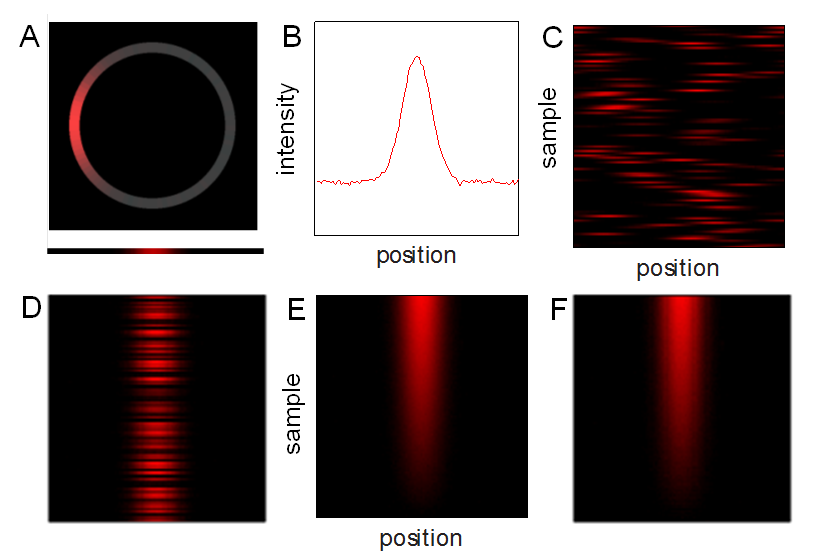
\includegraphics[width=8.4cm]{fig4}
\caption{(a) Set of vectors, each in a different orientation. The pariwise alignment angles are indicated. (b) The vectors from (a), each rotated so that the set is globally aligned. Note that the chosen rotation angles are consistent with the pairwise alignments in (a). (c) Data points (in black) which lie on a one-dimensional nonlinear curve in two dimensions. Each pair of data points is connected by an edge, and the edge weight is related to the Euclidean distance between the points through the diffusion kernel (see \eqref{eq:dmaps_W}), so that close data points are connected by dark (``stronger'') edges. (d) The data in (c), colored by the first (non-trivial) eigenvector from the diffusion map computational procedure, $\phi_2$. The color intensity is monotonic with the arclength, thus parameterizing the curve.  }
%\label{fig:schematics}
\customlabel{fig:schematics}{4}
\customlabel{subfig:synch1}{\ref{fig:schematics}a}
\customlabel{subfig:synch2}{\ref{fig:schematics}b}
\customlabel{subfig:dmaps_edges}{\ref{fig:schematics}c}
\customlabel{subfig:dmaps_color}{\ref{fig:schematics}d}
\end{figure}

Figure \ref{subfig:1d_aligned_unordered} shows the concentration profiles from Figure~\ref{subfig:1d_unaligned_unordered}, now aligned using angular synchronization.
%
It is reassuring that the peaks are aligned,
even though the algorithm uses no specific information about the existence or location of such peaks.
%
%We note once more that, since angular synchronization only uses pairwise rotation information,
%the optimal rotations are recovered up to a global rotation.

\subsection{Diffusion maps for temporal ordering}

After geometrically registering the data (concentration profiles or images), we want to order them in time to reconstruct the developmental dynamics.
%
%Our main assumption is that most of the variation in the data correlates with time.
%
We use diffusion maps \cite{coifman2005geometric}, a dimensionality reduction technique which aims to uncover low-dimensional, nonlinear structure in high-dimensional data sets, to temporally order our data.
%
Figure~\ref{subfig:dmaps_edges} shows an example of a two-dimensional data set (the ``high-dimensional" data) which lies on a one-dimensional nonlinear curve (the ``low-dimensional" manifold).
%
Figure~\ref{subfig:dmaps_color} shows the same data, now colored by the leading diffusion map coordinate.
%
The color parameterizes the one-dimensional curve that our eye can visually detect.
%
Our main assumptions are that our (one-dimensional profile, or two-dimensional image) data also lie on a one-dimensional, nonlinear curve, {\em and} that this curve is parameterized by time (e.g., in Figure~\ref{subfig:dmaps_color}, we assume that the data points are ordered from youngest to oldest along the curve).
%
Therefore, ordering data along this curve will effectively order data in time.
%
Because our data will be very high dimensional, we cannot do this by eye, and instead require an algorithm to automatically extract this one-dimensional structure.

To uncover a parameterization of this curve, we assume that data points which are close in the high-dimensional space should also be close {\em on the curve} (we would like images which look similar to be close together in our developmental trajectory).
%
%We therefore want to find a parameterization of the points, such that the points which are close in the original, high-dimensional space are {\em as close as possible} in the parameterization.
%
To emphasize this point, edges between the pairs of data points in Figure~\ref{subfig:dmaps_edges} are colored according to the distance between the data points, so that close data points have dark/strong
edges connecting them.
%
Visually, these dark edges delineate the one-dimensional curve; in contrast, the light edges are less informative
about the low-dimensional structure.
%
%We want points which are close in the high-dimensional space, i.e., connected by dark edges, to be close in our low-dimensional %parameterization.
%
Finding such a parameterization can be formulated as an optimization problem \cite{Belkin2003}, and the solution is given by the top (non-trivial) eigenvector of a Markov matrix which contains information about pairwise distances between the data points (see {\it Materials and Methods}).
%
This procedure has been named diffusion maps \cite{coifman2005geometric}.
%
%The formulation extends from curves to manifolds (i.e., we can search for an $n$-dimensional, rather than a one-dimensional, parameterization of the data, such that data points which are close in the high-dimensional space are also close in the $n$-dimensional parameterization).

Given our set of registered signals, shown in Figure \ref{subfig:1d_aligned_unordered}, we can use diffusion maps to order them in time.
%
We use the Euclidean distance between the (discretized in $\mathbb{R}^{100}$) aligned concentration profiles (the rows of Figure \ref{subfig:1d_aligned_unordered}) as our pairwise distances between data points.
%
Figure \ref{subfig:1d_aligned_ordered} shows the data from Figure \ref{subfig:1d_aligned_unordered}, now sorted by the value of the first (non-trivial) eigenvector, $\phi_2$.
%
As expected, the intensity of the peak grows as a function of $\phi_2$ (since we constructed these data
to have a peak growing in time).
%
%Although diffusion maps can order the data, it cannot tell us about the speed of this trajectory.
%
%Furthermore, the direction of the trajectory is also unknown; determining which end of the trajectory corresponds to the beginning of development is a task that needs to be done by hand.

\subsection{Vector diffusion maps for simultaneous registration and ordering}

%We are often interested in both registering and ordering our data.
%
%Our proposed alignment methodology, angular synchronization, utilizes the eigendecompostion of the matrix $H \in \mathbb{R}^{md \times md}$, and our proposed ordering algorithm, diffusion maps, utilizes the eigendecomposition of the matrix $A \in \mathbb{R}^{m \times m}$.
%
Angular synchronization (for registration) can be combined with diffusion maps (for temporal ordering) in a single eigencomputation that allows us to {\em simultaneously} recover the alignments {\em and} the temporal ordering.
%
This technique is called vector diffusion maps \cite{singer2012vector} (see {\it Materials and Methods}).
%
It both reduces the number of required eigencomputations, and is much more robust to noise, as mistakes in alignment are also considered when ordering the data.
%
Figure \ref{subfig:1d_aligned_ordered_vdm} shows the result of simultaneously registering and ordering the data in Figure \ref{subfig:1d_unaligned_unordered} using vector diffusion maps.
%
The data has been ordered by $\psi_{1, 3}$, the first (non-trivial) vector diffusion maps coordinate.

\subsection{Analysis of two-dimensional images}

The same methodologies (with small modifications) can be applied directly to our two-dimensional images.
%
Instead of one-dimensional profiles (discretized to $100$-dimensional concentration vectors), we now work with
two color, two-dimensional images (discretized into $100 \times 100$ pixels/$20000$-dimensional vectors), and we register the images with respect to translations and rotations (the symmetry group is $ISO(2)$).
%
To facilitate the application of vector diffusion maps, we approximate the two-dimensional translations and rotations by {\em three-dimensional rotations} (symmetry group $SO(3)$; see {\it Materials and Methods}, {\it SI Appendix}).
%
We use vector diffusion maps to align and order the images shown in Figure~\ref{subfig:images_unordered};
the results are shown in Figure~\ref{fig:images_ordered}.
%
Both the red and green peaks are now aligned, and the intensity of the red peaks grows as a function of the leading vector diffusion map coordinate.

In these experiments, we are fortunate enough to be able to validate our  automatic registration and ordering using prior physical knowledge about the system.
%
For registration, it is known that the peak in the distribution of Dorsal (shown in green) specifies the ventralmost position in the embryo, and that the nuclei (shown in gray) delineate the circumference of the embryo.
%%%
%%% maybe you can also quantify this guy
%%%
%
%Based on this, images can be translated to make the centers of the embryos coincide and rotated to place the peak of the green channel at the same angular position.
%
Temporal ordering, on the other hand, can be done based on the monotonic progress of cellularization (Figure~\ref{subfig:membranes}) \cite{figard2013plasma}.%; this helps validate our vector diffusion map-based ordering.
%
The results can be visually compared through the sequences of one-dimensional profiles (similar to the format in Figure~\ref{fig:1d_demo}), shown in Figures~\ref{subfig:1d_membranes}~and~\ref{subfig:1d_vdm}.
%
The general trends are consistent:
both green  and red peaks are aligned, and the red peaks grow as a function of time (or of the leading vector diffusion map coordinate).
%
However, Figure~\ref{subfig:1d_vdm}, which was automatically registered and ordered, shows an arguably better clustering of the ``outer" peaks in the top corners of the image.
%
%These peaks are more scrambled in Figure~\ref{fig:membrane_compare}b, which was analyzed using cellularization.
%
These peaks are known to arise later in development, and so it is reassuring that they appear at the end of the (recovered) trajectory.
%
%Furthermore, the membranes stop growing towards the end of this trajectory, making the ordering of the late signals in Figure~\ref{subfig:1d_membranes} less accurate.
%
Quantitatively, the rank correlation coefficient between these two temporal orderings is 0.9149, indicating that our automatic ordering is consistent with the ordering obtained from cellularization.

%Although our methods are fairly robust, they do require a sufficient amount of data so that DMAPS can ``see'' a smooth trajectory.
%
%We evaluated how much data is required by subsampling our data set (with replacement), and for each subsample, computing the temporal ordering using VDM and calculating the rank correlation between this ordering and the ordering from cellularization.
%
%The results are shown in Figure~\ref{subfig:bootstrap} (each data point is averaged over 50 random subsamples).
%
%For small data sets, the average rank correlation is very low, indicating that the orderings from VDM are inaccurate.
%
%However, for moderately sized data sets (approximately 30 data points), the rank correlation begins to plateau and VDM can accurately order the data.


\begin{figure}[t]
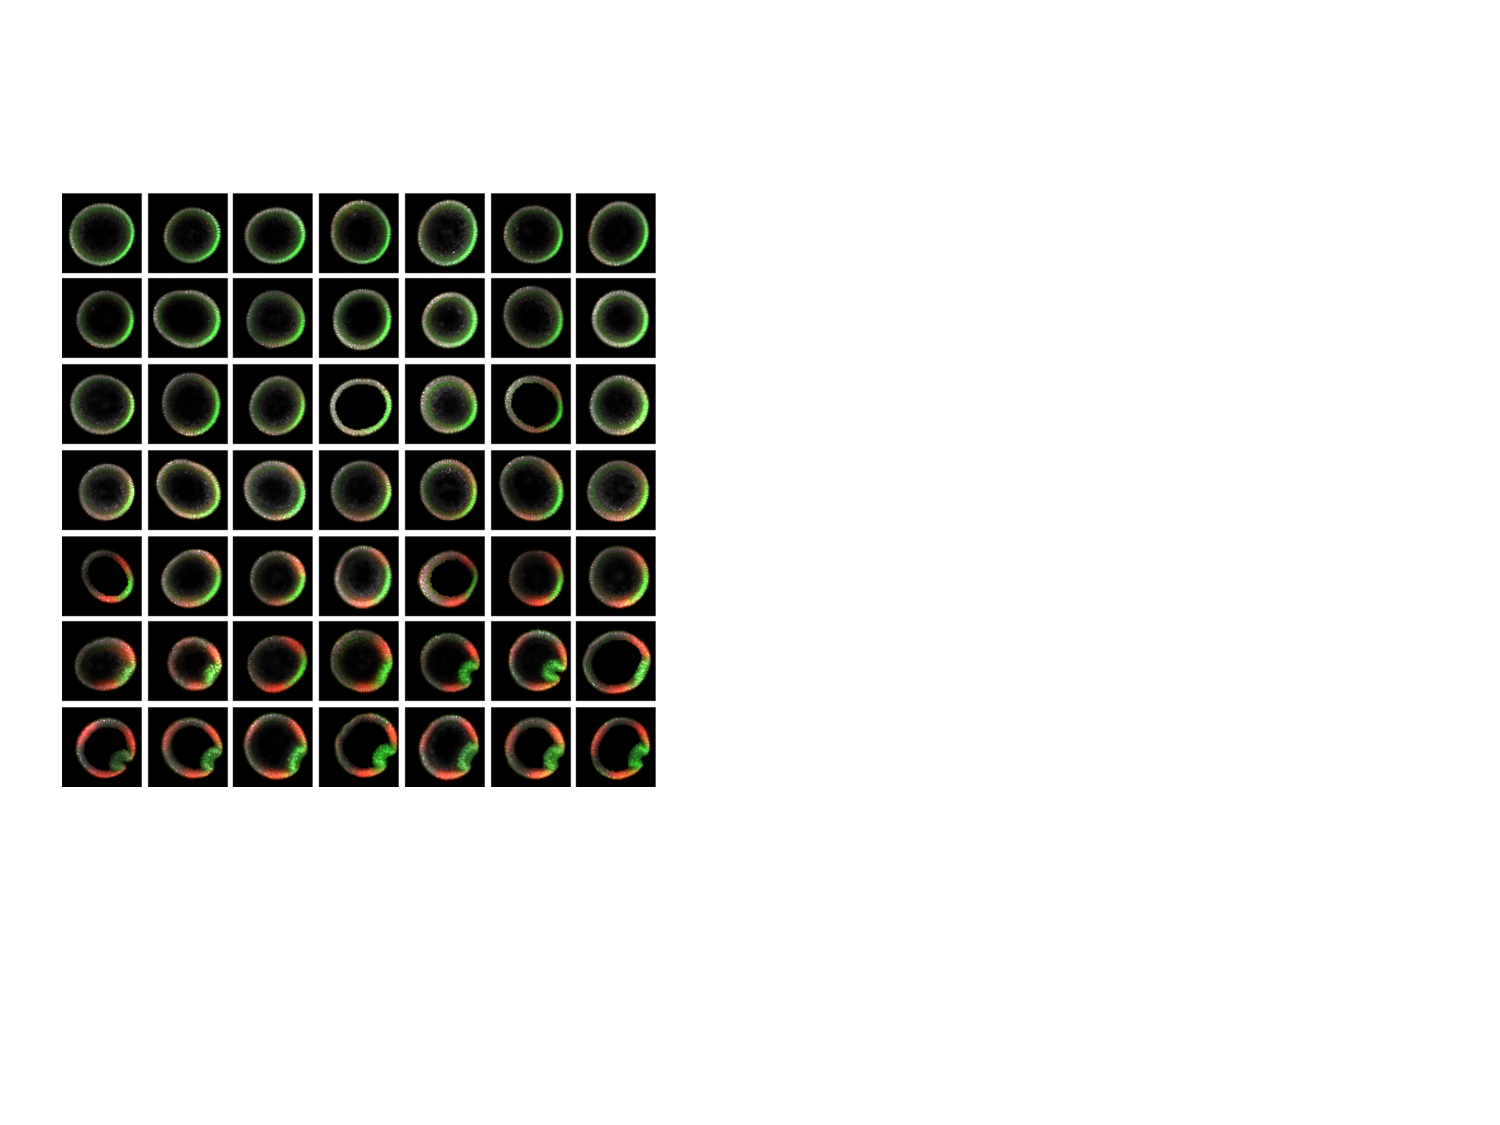
\includegraphics[width=8.4cm]{fig5}
\caption{The images in Figure~\ref{subfig:images_unordered}, aligned and temporally ordered using vector diffusion maps. The images are sorted according to the value of the first non-trivial vector diffusion maps component, $\psi_{1, 4}$.}
%\label{fig:images_ordered}
\customlabel{fig:images_ordered}{5}
\end{figure}

\begin{figure}[t]
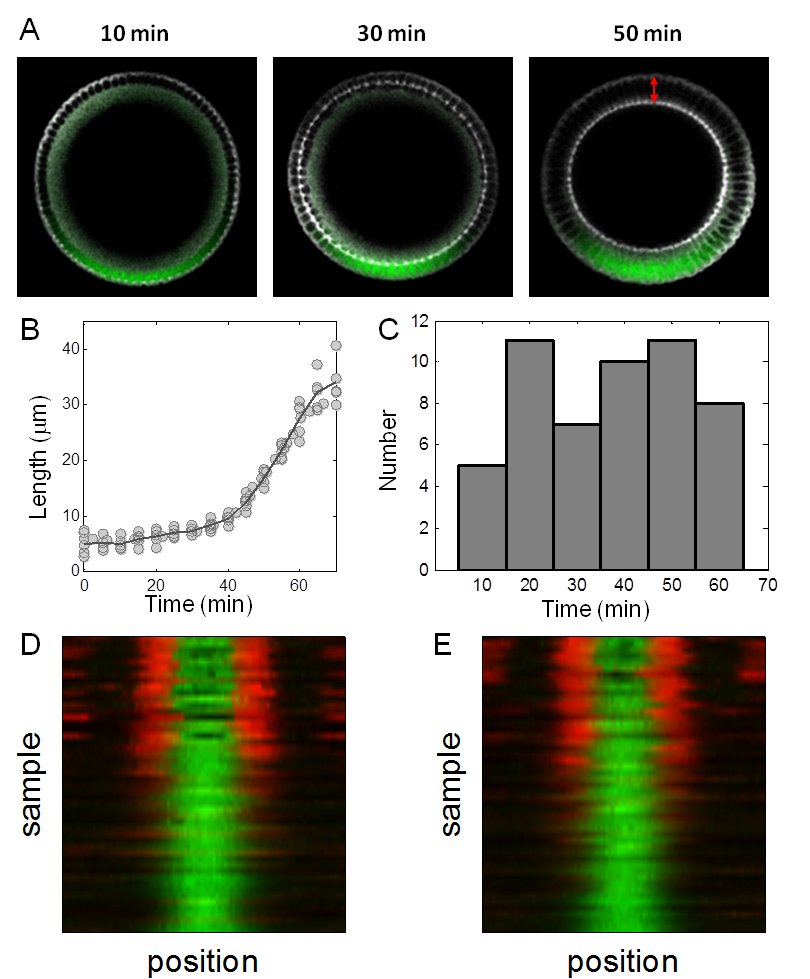
\includegraphics[width=8.4cm]{fig6}
\caption{(a) Images, stained for membranes (gray) and Dorsal (green) at different levels of development. (b) Membrane length as a function of time. The points correspoinding to the images in (a) are indicated with arrows. (c) The one-dimensional concentration profiles, registered by peak Dorsal fluorescence and ordered by membrane length. (d) The one-dimensional concentration profiles corresponding to the automatically registered and ordered images in Figure~\ref{fig:images_ordered}. }
%\label{fig:membrane_compare}
\customlabel{fig:membrane_compare}{6}
\customlabel{subfig:membranes}{\ref{fig:membrane_compare}a}
\customlabel{subfig:membrane_curve}{\ref{fig:membrane_compare}b}
\customlabel{subfig:1d_membranes}{\ref{fig:membrane_compare}c}
\customlabel{subfig:1d_vdm}{\ref{fig:membrane_compare}d}
\end{figure}

\section{Conclusions}

We have shown how symmetry and dimensionality reduction techniques can greatly accelerate the registration and temporal ordering of cross-sectional developmental imaging data.
%
Although we illustrated our methods using a specific data set from a study of {\em Drosophila} embryogenesis, the framework is quite general and requires little knowledge of the image features or the developmental dynamics.
%
To our knowledge, temporal ordering of {\em Drosophila} images has not been automated to this extent.
%
Recently, machine learning algorithms have been used to group {\em Drosophila} images into different developmental classes \cite{yuan2014automated}, yet there, the appropriate classes must be defined by the user and hand-labeled training data are required.

Temporal ordering of cross-sectional biological data has been studied in a variety of other contexts.
%
Cross-sectional RNA sequencing data has been temporally ordered \cite{anavy2014blind, trapnell2014dynamics}, where each data point is the transcriptome for a single sample.
%
Gene expression data from multiple patients has been studied in \cite{gupta2008extracting, qiu2011discovering};
here, each data point is a vector containing the expression levels of the various genes.
%
Snapshots of cells throughout the cell cycle can be described by a vector of features (e.g., amount of DNA) which quantify the cell's state  \cite{kafri2013dynamics}.
%
These problems are no different than our task of ordering images, each of which is a large vector of pixel intensities.
%
The majority of these works temporally order the data either by solving a traveling salesman problem on the data, or by constructing a minimum spanning tree of the data,
expecting that these structures (the path of the travelling salesman, or the minimum spanning tree) characterize the majority of the structure/variability within the data and provide an accurate picture of the dynamical progression.
%
We, instead, use diffusion maps, to construct a one-dimensional embedding of the data.
%
Diffusion maps are one of many nonlinear dimensionality reduction techniques that have been recently developed \cite{Belkin2003, tenenbaum2000global, Donoho2003, Roweis2000}.
%
They have been shown to be more robust to noise than other path-based algorithms, such as isomap \cite{balasubramanian2002isomap}, and so we suspect they may perform better than the ordering algorithms used in previous work.
%%%
%%%   we need help here
%%%
%
%Furthermore, although we use only the first diffusion maps coordinate to order the data (we assume the data are one-dimensional), diffusion maps are not limited to one-dimensional data and can be used to extract more complex structures.
%
%For example, in data which contains several branches or classes, the first few coordinates will delineate the branches or separate the classes.

The task of image registration has been widely studied, for applications such as face recognition \cite{rowley1998rotation}, medical image registration \cite{hajnal2010medical}, and texture classification \cite{greenspan1994rotation}.
%
The main point to note here is that many registration algorithms require the locations of landmarks or features within each image.
%
For example, in face recognition, the first step is often to find the eyes, nose, and mouth within the face, and then register images by aligning these features.
%
Images from a construction site over time have been temporally ordered, but these methods are also based on first identifying features within the images \cite{schindler2007inferring}.
%
In general, appropriate features may not be known {\em a priori}, and so we require a registration algorithm that does not rely on predefined features, but only on the inherent geometric symmetry of the problem.
%
Template-based methods are also common for registration, where one optimally aligns each image to a predefined template function.
%
However, these methods can suffer when the images are noisy, and the success of such methods can depend strongly on the template function \cite{shatsky2009method}.

Angular synchronization and vector diffusion maps require no feature points, and no template function.
%
These methods have been used to register two-dimensional cryo-electron microscopy images of three-dimensional molecules \cite{singer2011three}, where each image is a picture of (essentially) the {\em same} molecule; variation in the data comes from differences in the viewing angles (rotations of the molecule) and from instrument/measurement noise.
%
In contrast, our data contains variation from the different embryo orientations, as well as variation from the underlying developmental dynamics (which underpins the development of vector diffusion map algorithms).
%
%Other synchronization algorithms have been proposed \cite{bandeira2014multireference}.
%
These methods are formulated for general symmetry groups, and one might consider other symmetries, such as reflections and scaling/dilation.
%
The main requirement is that the symmetry group must be represented by orthogonal or unitary matrices \cite{singer2013spectral}.

Temporal ordering can also be accomplished without first registering the images, by constructing functions of the images which are invariant under translations and rotations. 
%
These functions are then used as the data in the diffusion maps calculation; since the functions do not change under translations and rotations, the resulting diffusion maps embedding is invariant to symmetries.
%
Such functions include the scattering transform \cite{mallat2012group} and the bispectrum \cite{zhao2014rotationally}.
%
These have the disadvantage that a we do not obtain a registered set of images, but only a temporal ordering of the images.
%
However, such methods can often be faster for large data sets, since the functions are computed per image, whereas synchronization requires the computation of all pairwise alignments.

In all of these data-driven methods, an essential question is how much and what type of data is needed to accurately reconstruct the dynamics.
%
For diffusion maps to temporally order the data, we require the developmental trajectory to be well-sampled, and that the principal direction of variability in the data (the coordinate which diffusion maps will recover) be monotonic in time.
%
In addition, the data should have spatial variability/structure for synchronization to successfully register the images.
%
In our example, the data set is sufficiently large so that the dynamics are well-sampled.
%
We have included both the red and the green channels so that the principal direction of variability is monotonic in time.
%
If we only used the green channel in our analysis, we could not temporally order the data using diffusion maps, as this signal does not change appreciably in time.
%
Both the red and green channels contain spatial variability: the green channel has one peak at a specific angular around the embryo, and the red channel has two peaks which grow in time.
%
This allows us to register the data points.
%
We include the green channel because the location of the red peaks is noisy, and so inclusion of the (less noisy) green channel allows us to more accurately register the images.
%
%For the methods we present here, we require a sufficient amount of data for the one-dimensional evolution curve to be ``seen'' by the algorithms (i.e., in Figure~\ref{subfig:dmaps_edges}, there are a sufficient number of data points so that our eye can see the curve; if there were only 4 data points, it would most likely be difficult for our eye to detect the one-dimensional structure).
%
%We also require the data to contain enough information so that the alignments and dynamics are apparent.
%
%For example, in the data presented in Figure~\ref{subfig:images_unordered}, the green peaks delineate the position of the ventral axis in the embryo, and the intensity of the red peaks grow over time.
%
%Therefore, these images contain information about rotational symmetries of the data as well as the dynamics of the data.
%
%If we removed the green signal, and only used the red signal in our analysis, the registration would not be as accurate.
%
%Furthermore, if we only used the green signal, then there would be no dynamic information (the shape or intensity of Dorsal does not change as a function of time in the developmental stage we are considering), and the temporal ordering would be inaccurate.
%
We are confident that for many applications, these requirements - data which adequately samples the developmental trajectory, and data with sufficient spatial and temporal variability - are easily met.
%
In these cases, our methods allow for the rapid, automated analysis of imaging data sets to help uncover complex dynamics and structure.


%%%   you should sample well enough in time
%%% your dmap coordinate should have a nice slope with time
%% you should have variation in angle ---and we know we are random in the rotations
%%
%% and now the green is an issue of noise.....
%% the green "sees" angle but not time,
%% the red sees angle and time, but angle badly
%% the ocmbination sees both well enough
%%
%%
%%   we need to say things about "other methods" -- Mallat, AmitNow, Procrustes...
%% and if we change the artificial stuff, but even if not
%% we need to say something about flips.
%% we need to say symmetry early at the beginning -- important
%%  the expression "factoring out symmetry", the reference to Ben....  something about symmetry groups 
%%    the smoothness when one wants to make movies.
%%  
%%
%%   Y is afraid of the compsci literature being "fairly represented"
%%
%%



%% == end of paper:

%% Optional Materials and Methods Section
%% The Materials and Methods section header will be added automatically.

%% Enter any subheads and the Materials and Methods text below.


\begin{materials}

\section{Angular synchronization for rotations\cite{singer2011angular}}

Let $x_1, \dots, x_m$ denote the signals that we wish to align with respect to rotations;
%
Each signal is a function defined on the unit circle (on the plane).
%
%Practically, it is discretized in a $n$-long vector (the local intensity at $n$ equidistant points around the circle);
%rotating the function by an angle $\theta$ then corresponds to cyclically shifting the elements of $x_i$ by $\frac{\theta_i}{2 \pi} n$ (rounded to the nearest integer to obtain a valid shift).
%
First assume that each signal $x_i$ is a {\em noisy} rotated copy of the underlying signal $x_{true}$
(which we are {\em not} given), such that
\begin{equation}
x_i = f(x_{true}, \theta_i) + \xi_i
\end{equation}
where the function $f(x_{true}, \theta_i)$ rotates the signal $x_{true}$ by $\theta_i$ radians, and $\xi_i$ is a (typically Gaussian) noise term.
%

Our goal is to obtain estimates of $\theta_1, \dots, \theta_m$.
%
Up to noise,
\begin{equation} \label{eq:pairwise_rot}
x_i \approx f(x_j, \theta_i - \theta_j) ;
\end{equation}
note that \eqref{eq:pairwise_rot} does not require knowledge of $x_{true}$.
%
We can obtain an {\em estimate} of $\theta_i - \theta_j$ by computing the rotation that optimally aligns $x_j$ to $x_i$,
i.e., %$\theta_{ij} \approx \theta_i - \theta_j$, where
%
\begin{equation} \label{eq:opt_angle}
\theta_i - \theta_j \approx \theta_{ij} = \argmin_{\theta} \|x_i - f(x_j, \theta)\|^2.
\end{equation}
%
Practically, the signals are discretized in a $n$-long vector (the local intensity at $n$ equidistant points around the circle);
rotating the function by an angle $\theta$ then corresponds to cyclically shifting the elements of $x_i$
by $\frac{\theta_i}{2 \pi} n$ (rounded to the nearest integer to obtain a valid shift).
%
For the one-dimensional discretized profiles shown in Figure~\ref{fig:1d_demo}, we exhaustively search over all $n=100$ possible shifts of the signals to compute the optimal angles in \eqref{eq:opt_angle}.
%
Alternatively, for continuous signals, an optimization algorithm
can be used to find the solution to \eqref{eq:opt_angle} \cite{ahuja2007template}.

Rather than work with the angles $\theta_{ij}$ directly, it is more convenient to consider work with the rotation matrices,
\begin{equation} \label{eq:R_theta}
R(\theta_{ij}) = \begin{bmatrix}
\cos(\theta_{ij}) & -\sin(\theta_{ij}) \\
\sin(\theta_{ij}) & \cos(\theta_{ij})
\end{bmatrix},
\end{equation}
which we can think of as operating on the points of the unit circle on which our signal is defined.
%
Successive rotations correspond to multiplication of the corresponding rotation matrices: $R(\alpha_1 + \alpha_2) = R(\alpha_1) R(\alpha_2)$.
%
Due to the orthogonality of rotation matrices, $R(-\alpha) = R(\alpha)^T$.

Let $d$ denote the dimension of the rotation matrices we are considering (for our example of planar rotations, $R(\theta_{ij}) \in \mathbb{R}^{2 \times 2}$ and $d=2$; we write our procedure for general $d$ because we will later consider three-dimensional rotations).
%
We construct the matrix $H \in \mathbb{R}^{md \times md}$, where $H$ is an $m \times m$ matrix of $d \times d$ blocks, with the $i,j^{th}$ block of $H$, $H_{ij}$, defined as
\begin{equation} \label{eq:H_to_R}
H_{ij} = R(\theta_{ij}).
\end{equation}
%
%
Under our assumption that $\theta_{ij} \approx \theta_i - \theta_j$, $H_{ij} \approx R(\theta_i) R(\theta_j)^T$
%\begin{equation}
%H_{ij} = R(\theta_{ij}) \approx R(\theta_i - \theta_j) = R(\theta_i) R(-\theta_j) = R(\theta_i) R(\theta_j)^T,
%\end{equation}
 and
\begin{equation} \label{eq:H_low_rank}
	H \approx
	\begin{bmatrix}
	R(\theta_1) \\
	R(\theta_2) \\
	\vdots \\
	R(\theta_m)
	\end{bmatrix}
	\begin{bmatrix}
	R(\theta_1)^T R(\theta_2)^T \dots R(\theta_m)^T
	\end{bmatrix}.
\end{equation}
%
It follows directly from \eqref{eq:H_low_rank}  that the top block eigenvector of $H$, %which we will denote $\hat{R}$,
contains our best estimates of $R(\theta_1), R(\theta_2), \dots, R(\theta_m)$.
%
Let $\phi_1, \phi_2, \dots, \phi_{md}$ denote the eigenvectors of $H$, ordered such that $|\lambda_1| \ge |\lambda_2| \ge \dots \ge |\lambda_{md}|$, where $\lambda_i$ is the eigenvalue corresponding to $\phi_i$.
%
Then,
\begin{equation}
\hat{R} =
\begin{bmatrix}
\hat{R}_1 \\
\hat{R}_2 \\
\vdots \\
\hat{R}_m
\end{bmatrix} =
\begin{bmatrix}
| & | & & | \\
\phi_1 & \phi_2 & \dots & \phi_d \\
| & | & & |
\end{bmatrix},
\end{equation}
where $\hat{R}_i \in \mathbb{R}^{d \times d}$ is the estimate for $R(\theta_i)$.
%
However, $\hat{R}_i$ is not guaranteed to be an orthogonal matrix;
the closest orthogonal matrix, $R_{i, est}$, is given by
\begin{equation} \label{eq:R_est}
R_{i, est} = U_i V_i^T,
\end{equation}
where $U_i$ and $V_i$ are the left and right singular vectors, respectively, of $\hat{R}_i$.
%
We adjust the sign of $\phi_1$ so that $det(R_{i, est}) = +1$, ensuring proper rotations.
%
We estimate $\theta_{i}$ by inverting \eqref{eq:R_theta}, and register the signals by rotating signal $i$ by $-\theta_i$.
%
We note that, in our actual computations, the pairwise rotations $\theta_{ij}$ are computed in a discrete setting, then the overall
synchronization is performed in the continuum context to obtain $\theta_i$, and the results are rounded to give the closest
discrete shift.

%Furthermore, this formulation also considers {\em higher-order} consistency information.
%
%For example, given our pairwise estimates $R_{ij}$, we know that relationships of the form
%\begin{equation} \label{eq:triplet_consistency}
%R(\theta_{ik}) R(\theta_{kj}) \approx R(\theta_i) R(\theta_k)^T R(\theta_k) R(\theta_j)^T = R(\theta_i) R(\theta_j)^T
%\end{equation}
%should also hold.
%
%Note that
%\begin{equation}
%(H^2)_{ij} = \sum_k R(\theta_{ik}) R(\theta_{kj});
%\end{equation}
%therefore, {\em all} infomation of the form in \eqref{eq:triplet_consistency} is contained in the matrix $H^2$.
%
%Because $H$ and $H^2$ have the same eigenvectors, our problem formulation accounts for not only pairwise alignment information, but also these higher-order considerations.

\section{Ordering using Diffusion Maps \cite{coifman2005geometric}}

Given $m$ data points $x_1, \dots, x_m$ (typically vectors in a high-dimensional space), we want to find a coordinate transformation $y(x)$ that preserves local information: points that are close in the original space should also be close in the coordinate $y$.
%
The first step is to construct the matrix $W \in \mathbb{R}^{m \times m}$, where $W_{ij}$ is large if points $x_i$ and $x_j$ are ``close.''
%
We use a diffusion kernel,
\begin{equation} \label{eq:dmaps_W}
%W_{ij} = \exp \left( -\frac{d^2(x_i, x_j)}{\epsilon^2} \right)
W_{ij} = e^{ -\frac{d^2(x_i, x_j)}{\epsilon^2}}
\end{equation}
where $d(x_i, x_j)$ is the pairwise distance between $x_i$ and $x_j$ (often the Euclidean distance), and $\epsilon$ is a characteristic scale.
%
Points less than $\epsilon$ apart are thus considered ``close'' and points farther than $\epsilon$ apart are considered ``far away''.
%
$\epsilon$ can be chosen using several techniques (see, for example \cite{coifman2008graph}); here, we take $\epsilon$ to be the median of the pairwise distances between data points.

We find a coordinate $y$ such that $y(x_i)$ and $y(x_j)$ are close if $W_{ij}$ is large by solving following optimization problem \cite{Belkin2003}
\begin{equation} \label{eq:dmaps_opt_problem}
\argmin_{y} \sum_{ij} W_{ij} (y(x_i) - y(x_j))^2
\end{equation}
%
To solve \eqref{eq:dmaps_opt_problem}, we compute the diagonal matrix $D$, where $D_{ii} = \sum_{j=1}^{m} W_{ij}$, and the matrix $A$, where
\begin{equation} \label{eq:dmaps_A}
A = D^{-1} W.
\end{equation}
%
We calculate the eigenvectors $\phi_1, \phi_2, \dots, \phi_m$ and eigenvalues $\lambda_1, \lambda_2, \dots, \lambda_m$ and order them such that $|\lambda_1| \ge |\lambda_2| \ge \dots \ge |\lambda_m|$.
%
%Because the matrix $A$ is similar to the symmetric matrix $D^{-1/2} W D^{-1/2}$, $A$ is guaranteed to have real eigenvalues and real, orthogonal eigenvectors.
%
Because the matrix $A$ is row-stochastic, $\lambda_1=1$ and $\phi_1$ is a constant vector; this is a trivial solution to \eqref{eq:dmaps_opt_problem}.
%
%In general, the next few eigenvectors $\phi_2, \dots, \phi_m$ give ``meaningful'' embedding coordinates for the data, such that $\phi_j(i)$ gives the $j^{th}$ embedding coordinate of the $i^{th}$ data point.
%
The next eigenvector, $\phi_2$, is the (non-trivial) solution to \eqref{eq:dmaps_opt_problem}, so that $\phi_2(j)$, the $j^{th}$ entry of $\phi_2$, gives the ``new" coordinate for data point $x_j$ (i.e., $\phi_2(j) = y(x_j)$).
%
In our application, we have assumed that this single direction of variability, parameterized by $\phi_2$, is one-to-one with time.
%
Ordering the data by $\phi_2(j)$ will then, effectively, order them in time.
%
The procedure generalizes when the data lie on higher-dimensional manifolds (not just curves) in data space.

\section{Vector Diffusion Maps \cite{singer2012vector}}

Given data points $x_1, \dots, x_m$, for vector diffusion maps, one first constructs the matrix $S \in \mathbb{R}^{md \times md}$, with the $i,j^{th}$ block of $S$, $S_{ij}$, defined as
\begin{equation} \label{eq:vdm_S}
	S_{ij} = A_{ij} H_{ij}
\end{equation}
%
where $A_{ij} \in \mathbb{R}$ (defined in \eqref{eq:dmaps_A}) pertains to the diffusion kernel between data points, and $H_{ij} \in \mathbb{R}^{d \times d}$ (defined in \eqref{eq:H_to_R}) pertains to the pairwise alignment between data points.
%
It is important to note that distance $d(x_i, x_j)$ used in the diffusion kernel in \eqref{eq:dmaps_W} is the distance between data points {\em after} after pairwise alignment, i.e., the minimum distance between all possible shifts of the two data points (which is obtained in \eqref{eq:opt_pairwise}).
%
In the language of symmetry groups, this distance is a metric between the orbits of the data points induced by the symmetry group.

One then computes the eigenvalues $\lambda_1, \lambda_2, \dots, \lambda_{md}$ and eigenvectors $\phi_1, \phi_2, \dots, \phi_{md}$ of $S$, and orders them such that $|\lambda_1| \ge |\lambda_2| \ge \dots \ge |\lambda_{md}|$.
%
These eigenvectors contain information about {\em both} the optimal rotations (the ``synchronization" component) and the
variation of the data {\em after} the spatial symmetries have been factored out - in our case, their temporal variation.
%
Assuming that the data (after symmetries have been factored out) are relatively closely clustered, it is reasonable
to expect, as in angular synchronization, that the top (block) eigenvector of $S$ contains approximations of the optimal rotations,
which can be computed in the same way from \eqref{eq:R_est}.
%
We then expect some subsequent eigenvector to contain information relevant to the ordering of the data,
i.e., about the main direction(s) of data variability modulo the geometric symmetries.
%%%
%%% somewhere we need to talk about compact groups
%%% discussion might be a good place because SCALING is obviously important and
%%% it is not compact......
%%%
%However, the eigenvectors now also contain information about the embedding coordinates for our images.
%
In general, the embedding coordinates will be given by
\begin{equation}
\psi_{k,l} (i) = \langle \phi_k(i), \phi_l(i) \rangle
\end{equation}
where $\phi_k(i) \in \mathbb{R}^d$ denotes the $i^{th}$ block of $\phi_k$.
%
If we assume that our data mainly vary along a one-dimensional manifold, and that the rotations and the dynamics are uncoupled and therefore separable, one expects the embedding coordinate for our data %(i.e., the analog of $\phi_2$ from the diffusion maps case)
to be  $\psi_{1,d+1}$.
%
Our example is, by physical considerations, a separable one; if no separability claims can be made, a second diffusion map step, using $\psi_{k,l}$ as the coordinates, may uncover a
useful parameterization of the data manifold modulo symmetries.
%%%
%%% \cite....
%%%

\section{Registering Images with Respect to Translations and Rotations} \label{subsec:trans_rot_register}

Registering images with respect to rotations {\em and translations} requires some additional care.
%
%We are not only interested in registering the one-dimensional concentration profiles with respect to rotational symmetries, but we would also like to register the two-dimensional images shown in Figure \ref{fig:fluorescent_images} with respect to rotations {\em and} translations.
%
%We first compute the translations and rotations to optimally align each pair of data points.
%
Practically, we have planar square images discretized as pixels (rather than continuous functions on the plane).
%
We therefore solve discrete pairwise optimization problems: for each image pair $I_i$ and $I_j$ we find
\begin{equation}\label{eq:opt_pairwise}
(\theta_{ij}, dx_{ij}, dy_{ij}) = \argmin_{
\scriptsize \begin{matrix}
\theta \in [0, 2\pi) \\
dx, dy \in [-\Delta, \Delta]\\
%dy \in [-\Delta, \Delta]
\end{matrix}
} \|g(I_j, \theta, dx, dy) - I_i \|^2.
\end{equation}
where $g(I_j, \theta, dx, dy)$ is the image that results from first rotating the image $I_j$ around the center of the square by $\theta$ degrees, then translating the resulting
image by $dx$ pixel widths in the $x$ direction, and finally translating by $dy$ pixel widths in the $y$ direction.
%
The norm we use, $\| \cdot \|$, is the Euclidean norm between the pixel intensities for both the red and green channels.
%
The domain of the image (a square) is not invariant to our rotations and translations; however, the pixels close to the border of the square have zero intensity, and so the norm can be computed as long as the main image (the embryo) does not move out of the original square.
%
%The norm \eqref{eq:opt_pairwise} involve an integral over the square, which is not left invariant by our rotations and
%translations; noting however that the pixels close to the border of the square have zero intensity allows a meaningful
%computation of this norm as long as the ``main feature" (the embryo) does not move out of the original square (no ``corner effects").
%
This also justifies the $\Delta$ limits in the translation: 
in \eqref{eq:opt_pairwise}, $\Delta$ is chosen such that only edge pixels with little to no signal are shifted, and the main image is not split or separated when translating (we take $\Delta=20$, which corresponds to a 20\% shift in the image).%; it does not make sense to shift the images so much that
%the embryo would ``move out" of the original square.
%
Image rotation is performed with the \texttt{imrotate} function in Matlab, using nearest neighbor interpolation to estimate the pixel intensities after rotation.
%, since there is no direct mapping of the pixels of the unrotated image to the pixels of the rotated image.
%
The missing pixels in the rotated image are taken to have zero intensity.
%
The translations are implemented by shifting the pixels (for computational speed, we used periodic boundary conditions).
%
We only consider shifts that correspond to an integer number of pixels, to remove the need for interpolation when doing the translations.
%
The solution to \eqref{eq:opt_pairwise} is not easily computed, as the objective function will most likely be nonconvex.
%
Therefore, instead of using an optimization procedure, we discretize the search space and exhaustively search to find the solution.
%
Our discrete translation steps are $1/10^{th}$ of the domain, and our discrete rotations steps are $1/20^{th}$ of $2 \pi$. 
%
%We discritize the search space of rotations into 20 possible rotations %($d\theta  \in \{0, \pi/10, \pi/5, \dots, 9 \pi/5, 19\pi/10 \}$),
%and 11 possible translations in both . %($dx, dy \in \{-20, -16, -12, \dots, 12, 16, 20 \}$).
%
We check all possible combinations for the rotation and translations that best align $I_j$ to $I_i$.
%
Although computationally demanding, this ``embarrassingly parallelizable" direct enumeration approach is not prohibitive.
%
%Although this can be somewhat time intensive, it is not prohibitive for the data sets we consider, and can be trivially parallelized if necessary.
%
%The solution will not be the exact solution to \eqref{eq:opt_pairwise}, but it will (most likely) be a close approximation.
%
%Since our techniques are robust to noise, close approximations will be sufficient to obtain accurate results.

%As discussed above, for angular synchronization, the underlying symmetry group needs to have a real and orthogonal matrix representation.
%
%We therefore convert $ISO(2)$, the group of two-dimensional translations and rotations, to $SO(3)$, the group of three-dimensional rotations.
%

The requirements for the synchronization algorithm (i.e., for \eqref{eq:H_low_rank} to be satisfied) include the condition that the matrices used to represent the symmetry group be orthogonal \cite{singer2013spectral}.
%
However, the typical matrix representation for $ISO(2)$, the group of two-dimensional translations and rotations, does not satisfy this property.
%
Instead, we {\em approximately} represent rotations and translations in two-dimensions using {\em three-dimensional rotation matrices}, by projecting the (two-dimensional) image onto a portion of the surface of a (three-dimensional) sphere \cite{singer2011angular} (see {\it SI Appendix}).
%
Rotation of the image corresponds to rotation around one principal axis in three dimensions, while translation of the image corresponds (approximately) to rotations around the other two principal axes. %(Clearly, not all translations can be described this way, as translations can range from $-\infty$ to $+ \infty$, and rotations are only from $0$ to $2 \pi$. However, the images we will be considering are already mostly centered, and so we are only interested in small translations that are well within the $[0, 2\pi)$ range.)
%
%These rotation matrices are (by definition) orthogonal, and successive applications of various translations and rotations can be described via multiplication of the corresponding rotation matrices in $SO(3)$.

To convert the optimal two-dimensional translation and rotation to corresponding (continuous) three-dimensional rotations,
we first compute the Euler angles $\alpha_{ij}$, $\beta_{ij}$, and $\gamma_{ij}$,
\begin{equation} \label{eq:angle_relations}
%\begin{aligned}
%	\alpha_{ij} &= \theta_{ij} \\
%	\beta_{ij} &= \frac{dx_{ij}}{n} \times \eta_{proj} \\
%	\gamma_{ij} &= \frac{dy_{ij}}{n} \times \eta_{proj} \\
%\end{aligned}
	\alpha_{ij} = \theta_{ij}, \; \; \;
	\beta_{ij} = \frac{dx_{ij}}{n} \times \eta_{proj}, \; \; \;
	\gamma_{ij} = \frac{dy_{ij}}{n} \times \eta_{proj}
\end{equation}
where $\eta_{proj}$ is the angular portion of the sphere onto which we choose to project the image.
%
We take $\eta_{proj} =  \pi/8$, so the image lies on a $\pi/8 \times \pi/8$ radians portion of the unit sphere;
this portion of the sphere is small enough so that curvature effects are not prominent in the image.
%
We write rotations around the three principal axes, $R^x(\alpha)$, $R^y(\beta)$, and $R^z(\gamma)$, in terms of the three Euler angles
%\small
\begin{equation}
\begin{aligned}
	R^x(\alpha) &= \begin{bmatrix}
	1 & 0 & 0 \\
    0 & \cos(\alpha) & -\sin(\alpha) \\
    0 & \sin(\alpha) & \cos(\alpha)
	\end{bmatrix} \\
	R^y(\beta) &= \begin{bmatrix}
	\cos(\beta) & 0 & \sin(\beta) \\
    0 & 1 & 0 \\
    -\sin(\beta) & 0 & \cos(\beta)
    \end{bmatrix} \\
	R^z(\gamma) &= \begin{bmatrix}
	\cos(\gamma) & -\sin(\gamma) & 0 \\
    \sin(\gamma) & \cos(\gamma) & 0 \\
    0 & 0 & 1
    \end{bmatrix}.
\end{aligned}
\end{equation}
%\normalsize
%
The total rotation, $R_{ij} \in SO(3) \subset \mathbb{R}^{3 \times 3}$, is
\begin{equation} \label{eq:total_rot}
	R(\alpha_{ij}, \beta_{ij}, \gamma_{ij})	 = R^z(\gamma_{ij})  R^y(\beta_{ij})  R^x(\alpha_{ij}).
%R(\alpha_{ij}, \beta_{ij}, \gamma_{ij}) =
%\begin{bmatrix}
%\cos(\beta) \cos(\gamma) & \cos(\gamma)\sin(\alpha)\sin(\beta)-\cos(\alpha) \sin(\gamma) & \cos(\alpha)\cos(\gamma)\sin(\beta)+ \sin(\alpha)\sin(\gamma) \\
%\cos(\beta) \sin(\gamma) & \cos(\alpha) \cos(\gamma)+\sin(\alpha) \sin(\beta) \sin(\gamma) & \cos(\alpha) \sin(\beta) \sin(\gamma)-\cos(\gamma) \sin(\alpha) \\
%-\sin(\beta) & \cos(\beta) \sin(\alpha) & \cos(\alpha) \cos(\beta))
%\end{bmatrix}
\end{equation}
%
%\eqref{eq:total_rot} corresponds to first rotating the image by $\theta$, then translating the image by $dx$ pixels in the $x$ direction, and finally translating the image by $dy$ pixels in the $y$ direction (we note that, because the rotation matrices operate from the left, the rightmost rotation matrix in the product in \eqref{eq:total_rot} corresponds to the first operation we perform on the image).

These rotation matrices $R(\alpha_{ij}, \beta_{ij}, \gamma_{ij})$ are used in formulating the matrix $H$ in \eqref{eq:H_to_R} for angular synchronization, or the matrix $S$ in \eqref{eq:vdm_S} for vector diffusion maps.
%
We can then compute the (approximately) optimal rotations (and, in the case of vector diffusion maps, temporal orderings) for the images.
%
From the three-dimensional rotations $R_{1, est}, \dots, R_{m, est}$, we  require the corresponding translations and rotations of the images.
%
We first multiply all rotations by $R_{1, est}^T$ to ensure that all the images are (approximately) in the region of the sphere where we began;
$R_{i,est}^T$ then gives the rotation matrix which registers image $i$.
%
From a rotation matrix $R$, we compute the Euler angles $\alpha$, $\beta$, and $\gamma$ using the following relationships
\begin{equation}
\begin{aligned}
R_{1,1} & = \cos(\beta)\cos(\gamma) &
R_{2,1} & = \cos(\beta)\sin(\gamma) \\
R_{3,1} & = -\sin(\beta) &
R_{3,2} & = \sin(\alpha)\cos(\beta) \\
R_{3,3} & = \cos(\alpha)\cos(\beta)  &
\end{aligned}
\end{equation}
%
Inverting \eqref{eq:angle_relations} yields the corresponding approximate translations and rotation, and we round optimal translations to the nearest integer to remove the need for interpolation when translating the images.

\end{materials}


%% Optional Appendix or Appendices
%% \appendix Appendix text...
%% or, for appendix with title, use square brackets:
%% \appendix[Appendix Title]


\begin{acknowledgments}
- text of acknowledgments here, including grant info -
\end{acknowledgments}

%% PNAS does not support submission of supporting .tex files such as BibTeX.
%% Instead all references must be included in the article .tex document.
%% If you currently use BibTeX, your bibliography is formed because the
%% command \verb+\bibliography{}+ brings the <filename>.bbl file into your
%% .tex document. To conform to PNAS requirements, copy the reference listings
%% from your .bbl file and add them to the article .tex file, using the
%% bibliography environment described above.

%%  Contact pnas@nas.edu if you need assistance with your
%%  bibliography.

% Sample bibliography item in PNAS format:
%% \bibitem{in-text reference} comma-separated author names up to 5,
%% for more than 5 authors use first author last name et al. (year published)
%% article title  {\it Journal Name} volume #: start page-end page.
%% ie,
% \bibitem{Neuhaus} Neuhaus J-M, Sitcher L, Meins F, Jr, Boller T (1991)
% A short C-terminal sequence is necessary and sufficient for the
% targeting of chitinases to the plant vacuole.
% {\it Proc Natl Acad Sci USA} 88:10362-10366.


%% Enter the largest bibliography number in the facing curly brackets
%% following \begin{thebibliography}

\bibliographystyle{pnas}
\bibliography{background_reading/references,../../references/references}

%\begin{thebibliography}{}

%\end{thebibliography}


\end{article}
%%%%%%%%%%%%%%%%%%%%%%%%%%%%%%%%%%%%%%%%%%%%%%%%%%%%%%%%%%%%%%%%

%% Adding Figure and Table References
%% Be sure to add figures and tables after \end{article}
%% and before \end{document}

%% For figures, put the caption below the illustration.
%%
%% \begin{figure}
%% \caption{Almost Sharp Front}\label{afoto}
%% \end{figure}

%% For Tables, put caption above table
%%
%% Table caption should start with a capital letter, continue with lower case
%% and not have a period at the end
%% Using @{\vrule height ?? depth ?? width0pt} in the tabular preamble will
%% keep that much space between every line in the table.

%% \begin{table}
%% \caption{Repeat length of longer allele by age of onset class}
%% \begin{tabular}{@{\vrule height 10.5pt depth4pt  width0pt}lrcccc}
%% table text
%% \end{tabular}
%% \end{table}

%% For two column figures and tables, use the following:

%% \begin{figure*}
%% \caption{Almost Sharp Front}\label{afoto}
%% \end{figure*}

%% \begin{table*}
%% \caption{Repeat length of longer allele by age of onset class}
%% \begin{tabular}{ccc}
%% table text
%% \end{tabular}
%% \end{table*}


%\begin{figure*}
%\begin{subfigure}{0.2\textwidth}
%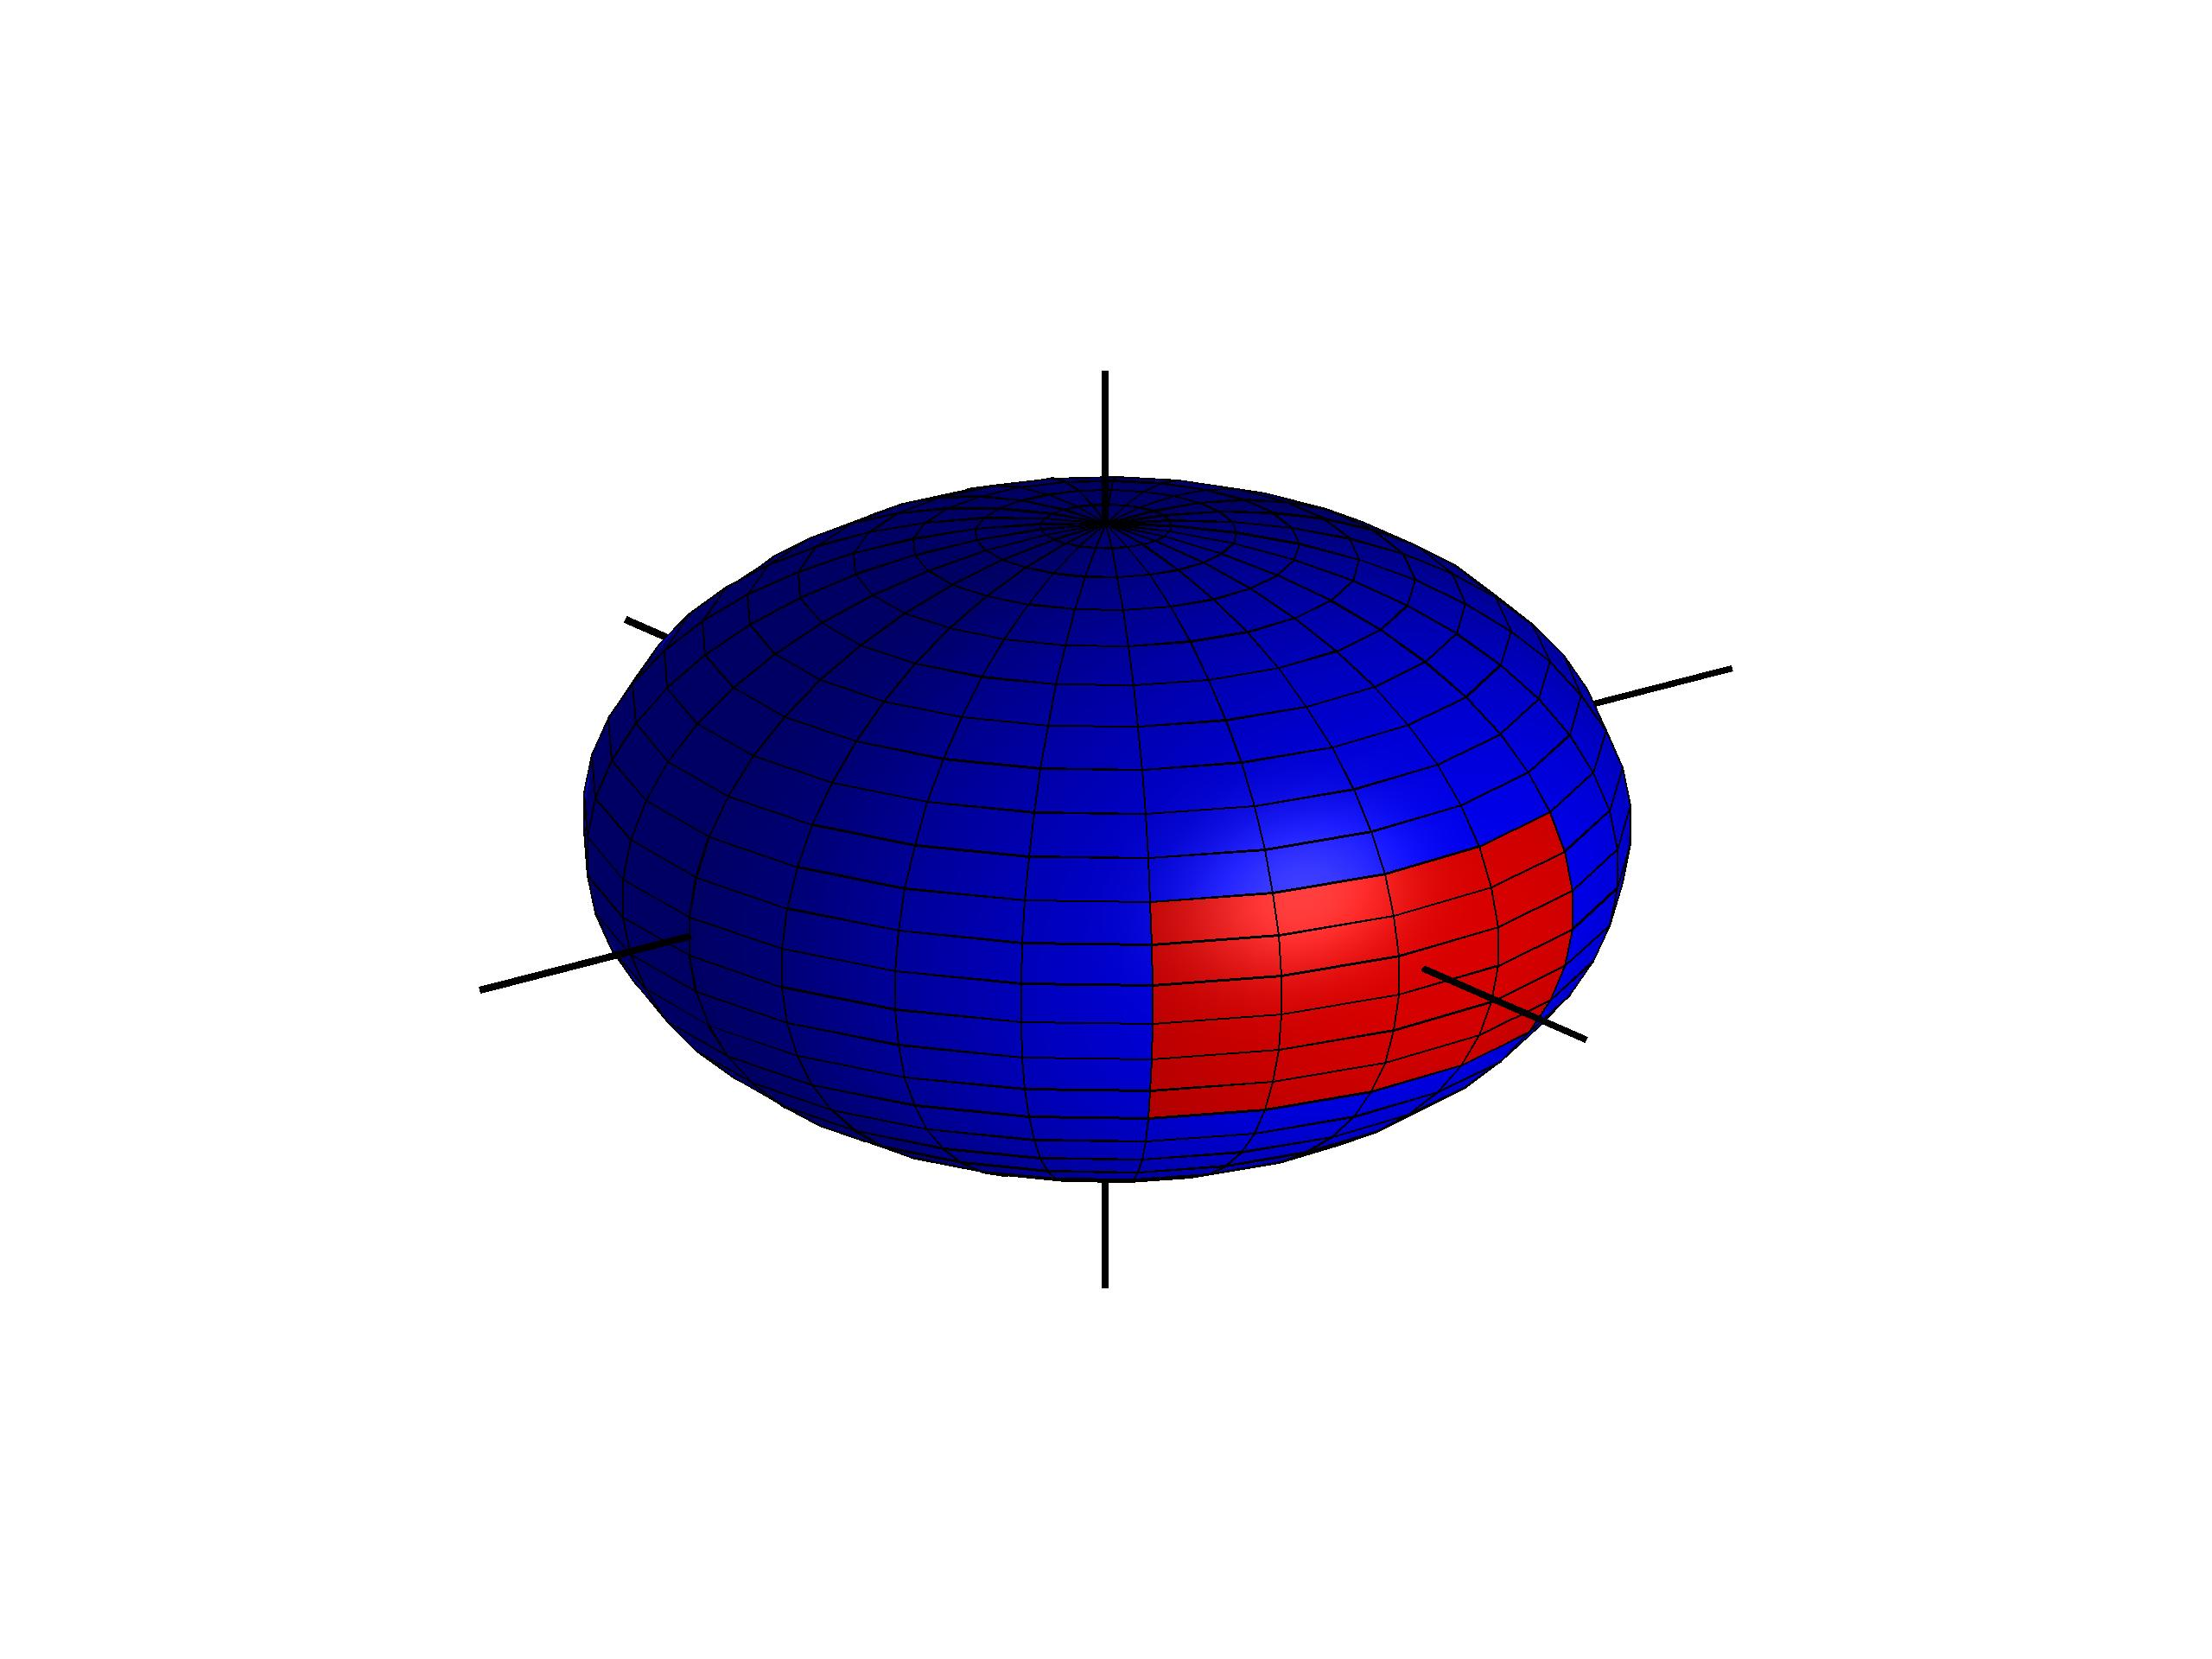
\includegraphics[width=\textwidth]{sphere_1}
%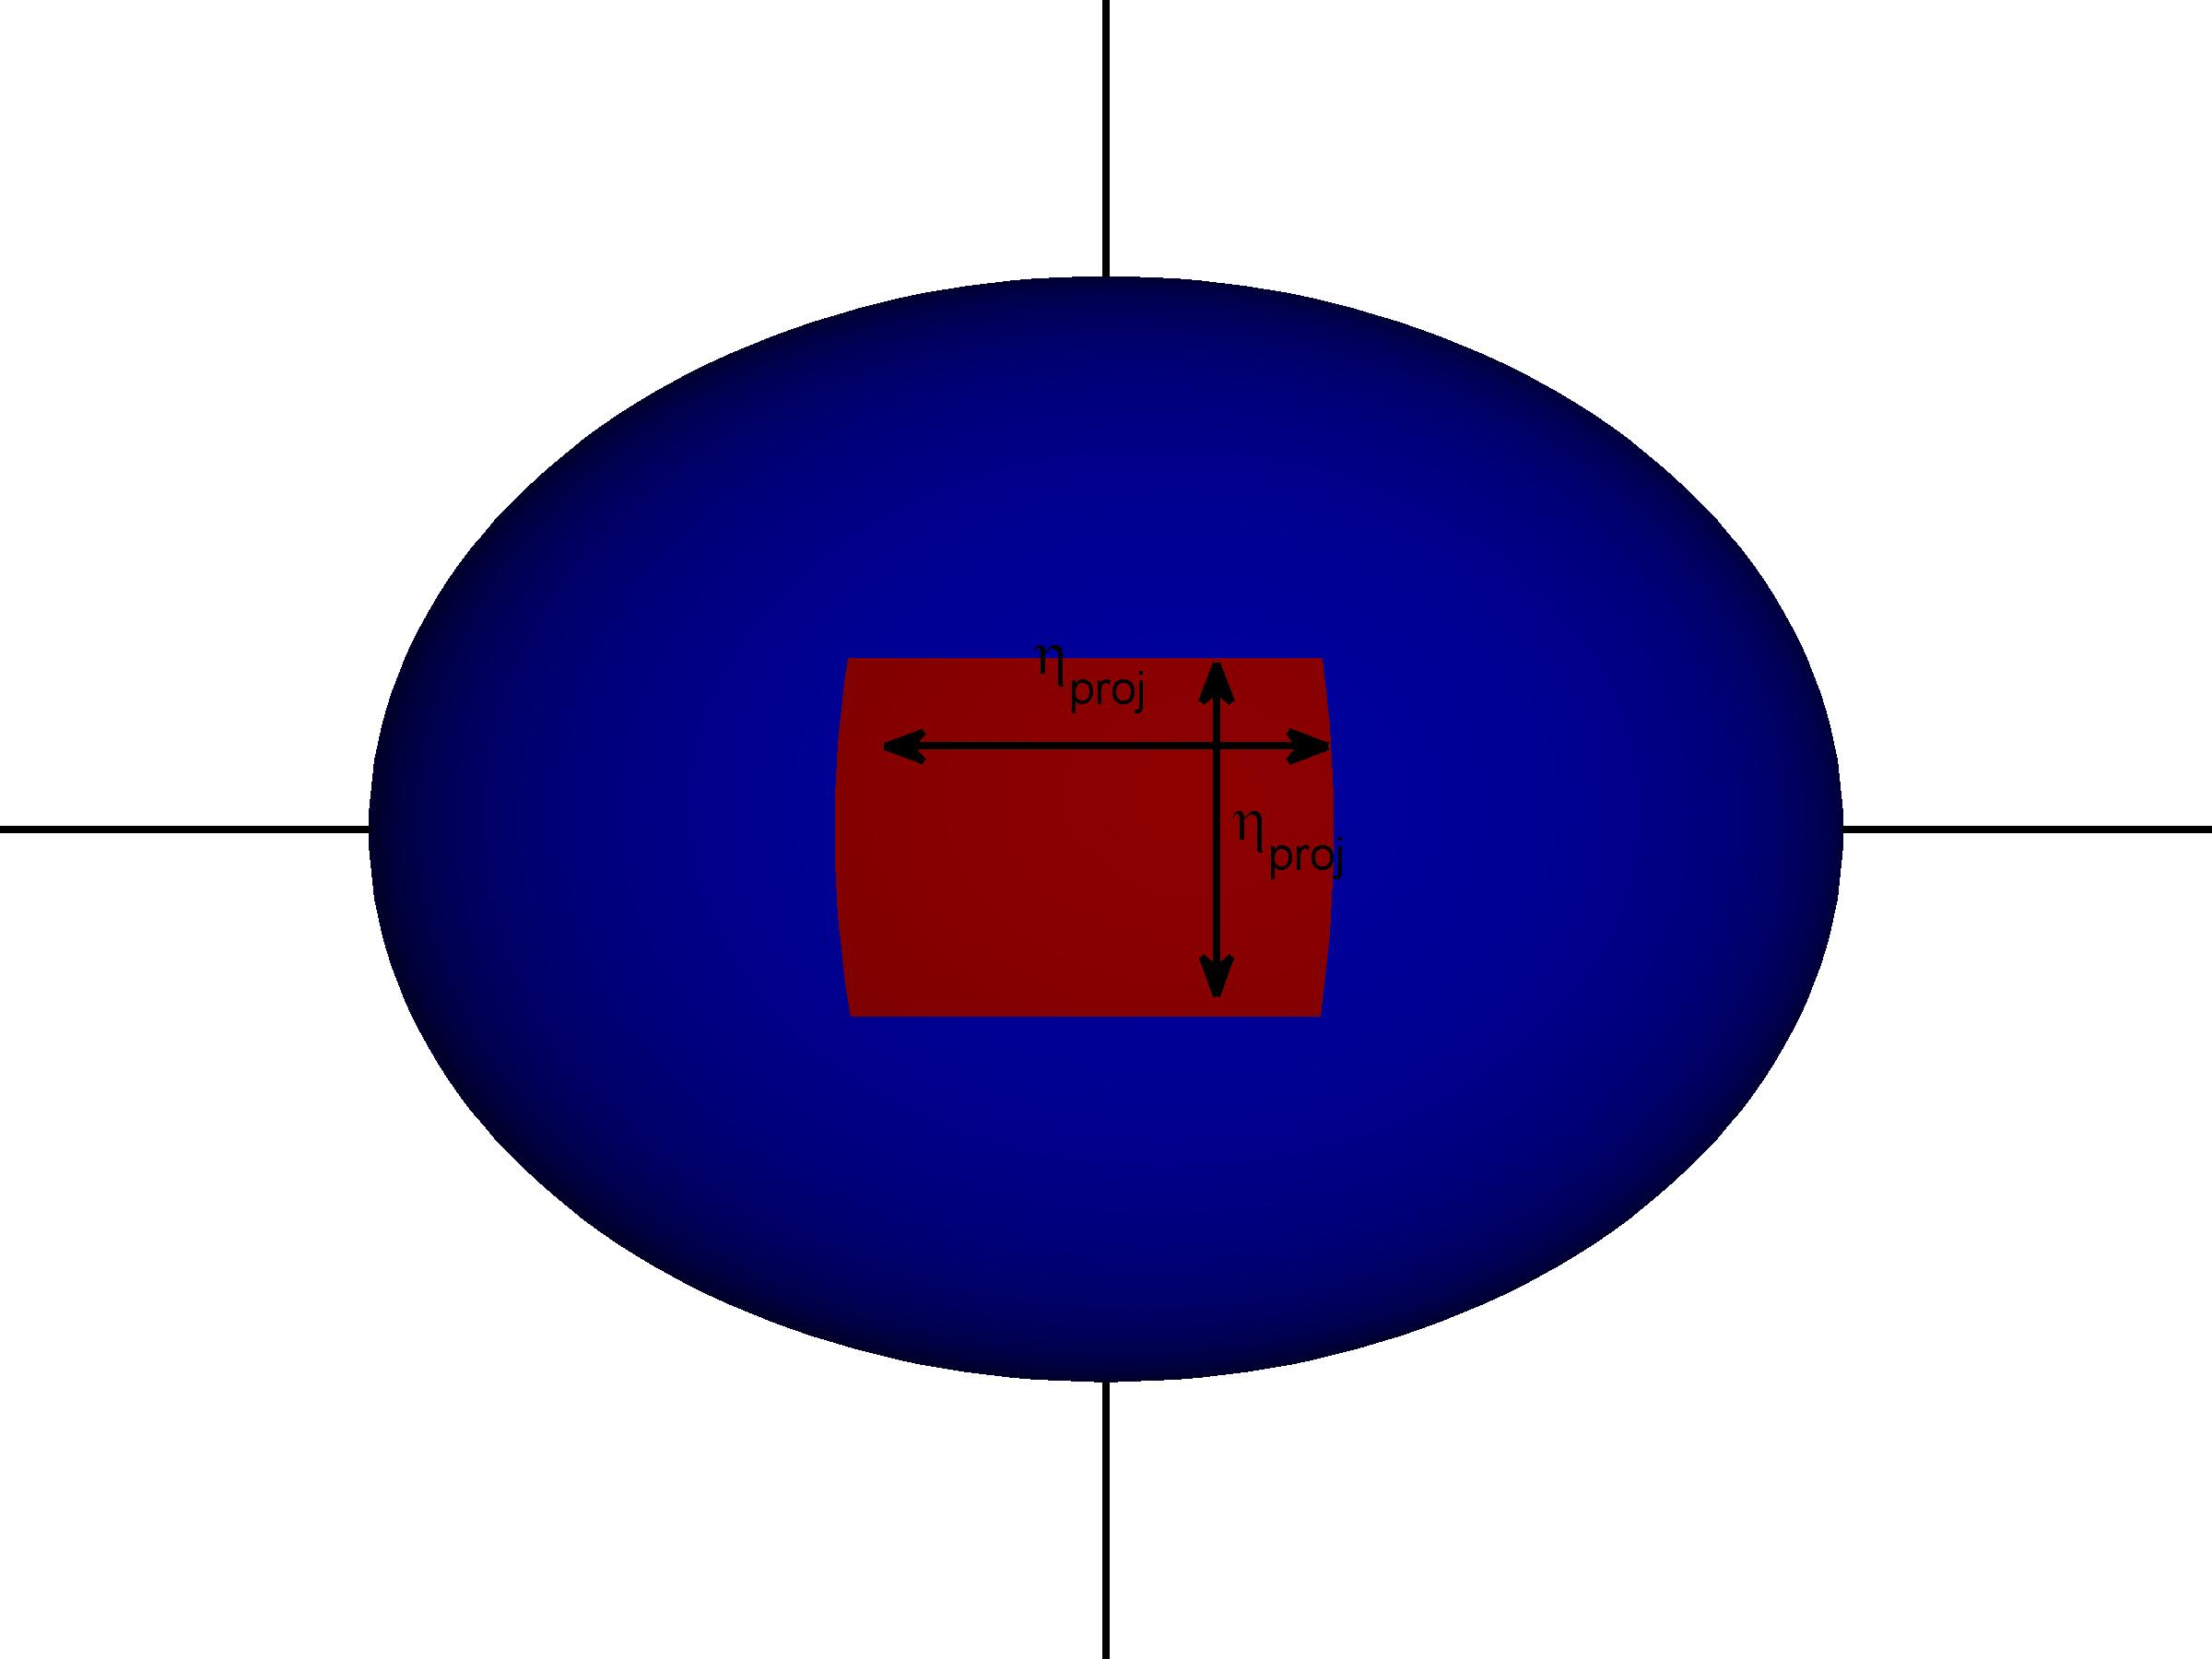
\includegraphics[width=\textwidth]{sphere2_1}
%\caption{}
%\end{subfigure}
%\begin{subfigure}{0.2\textwidth}
%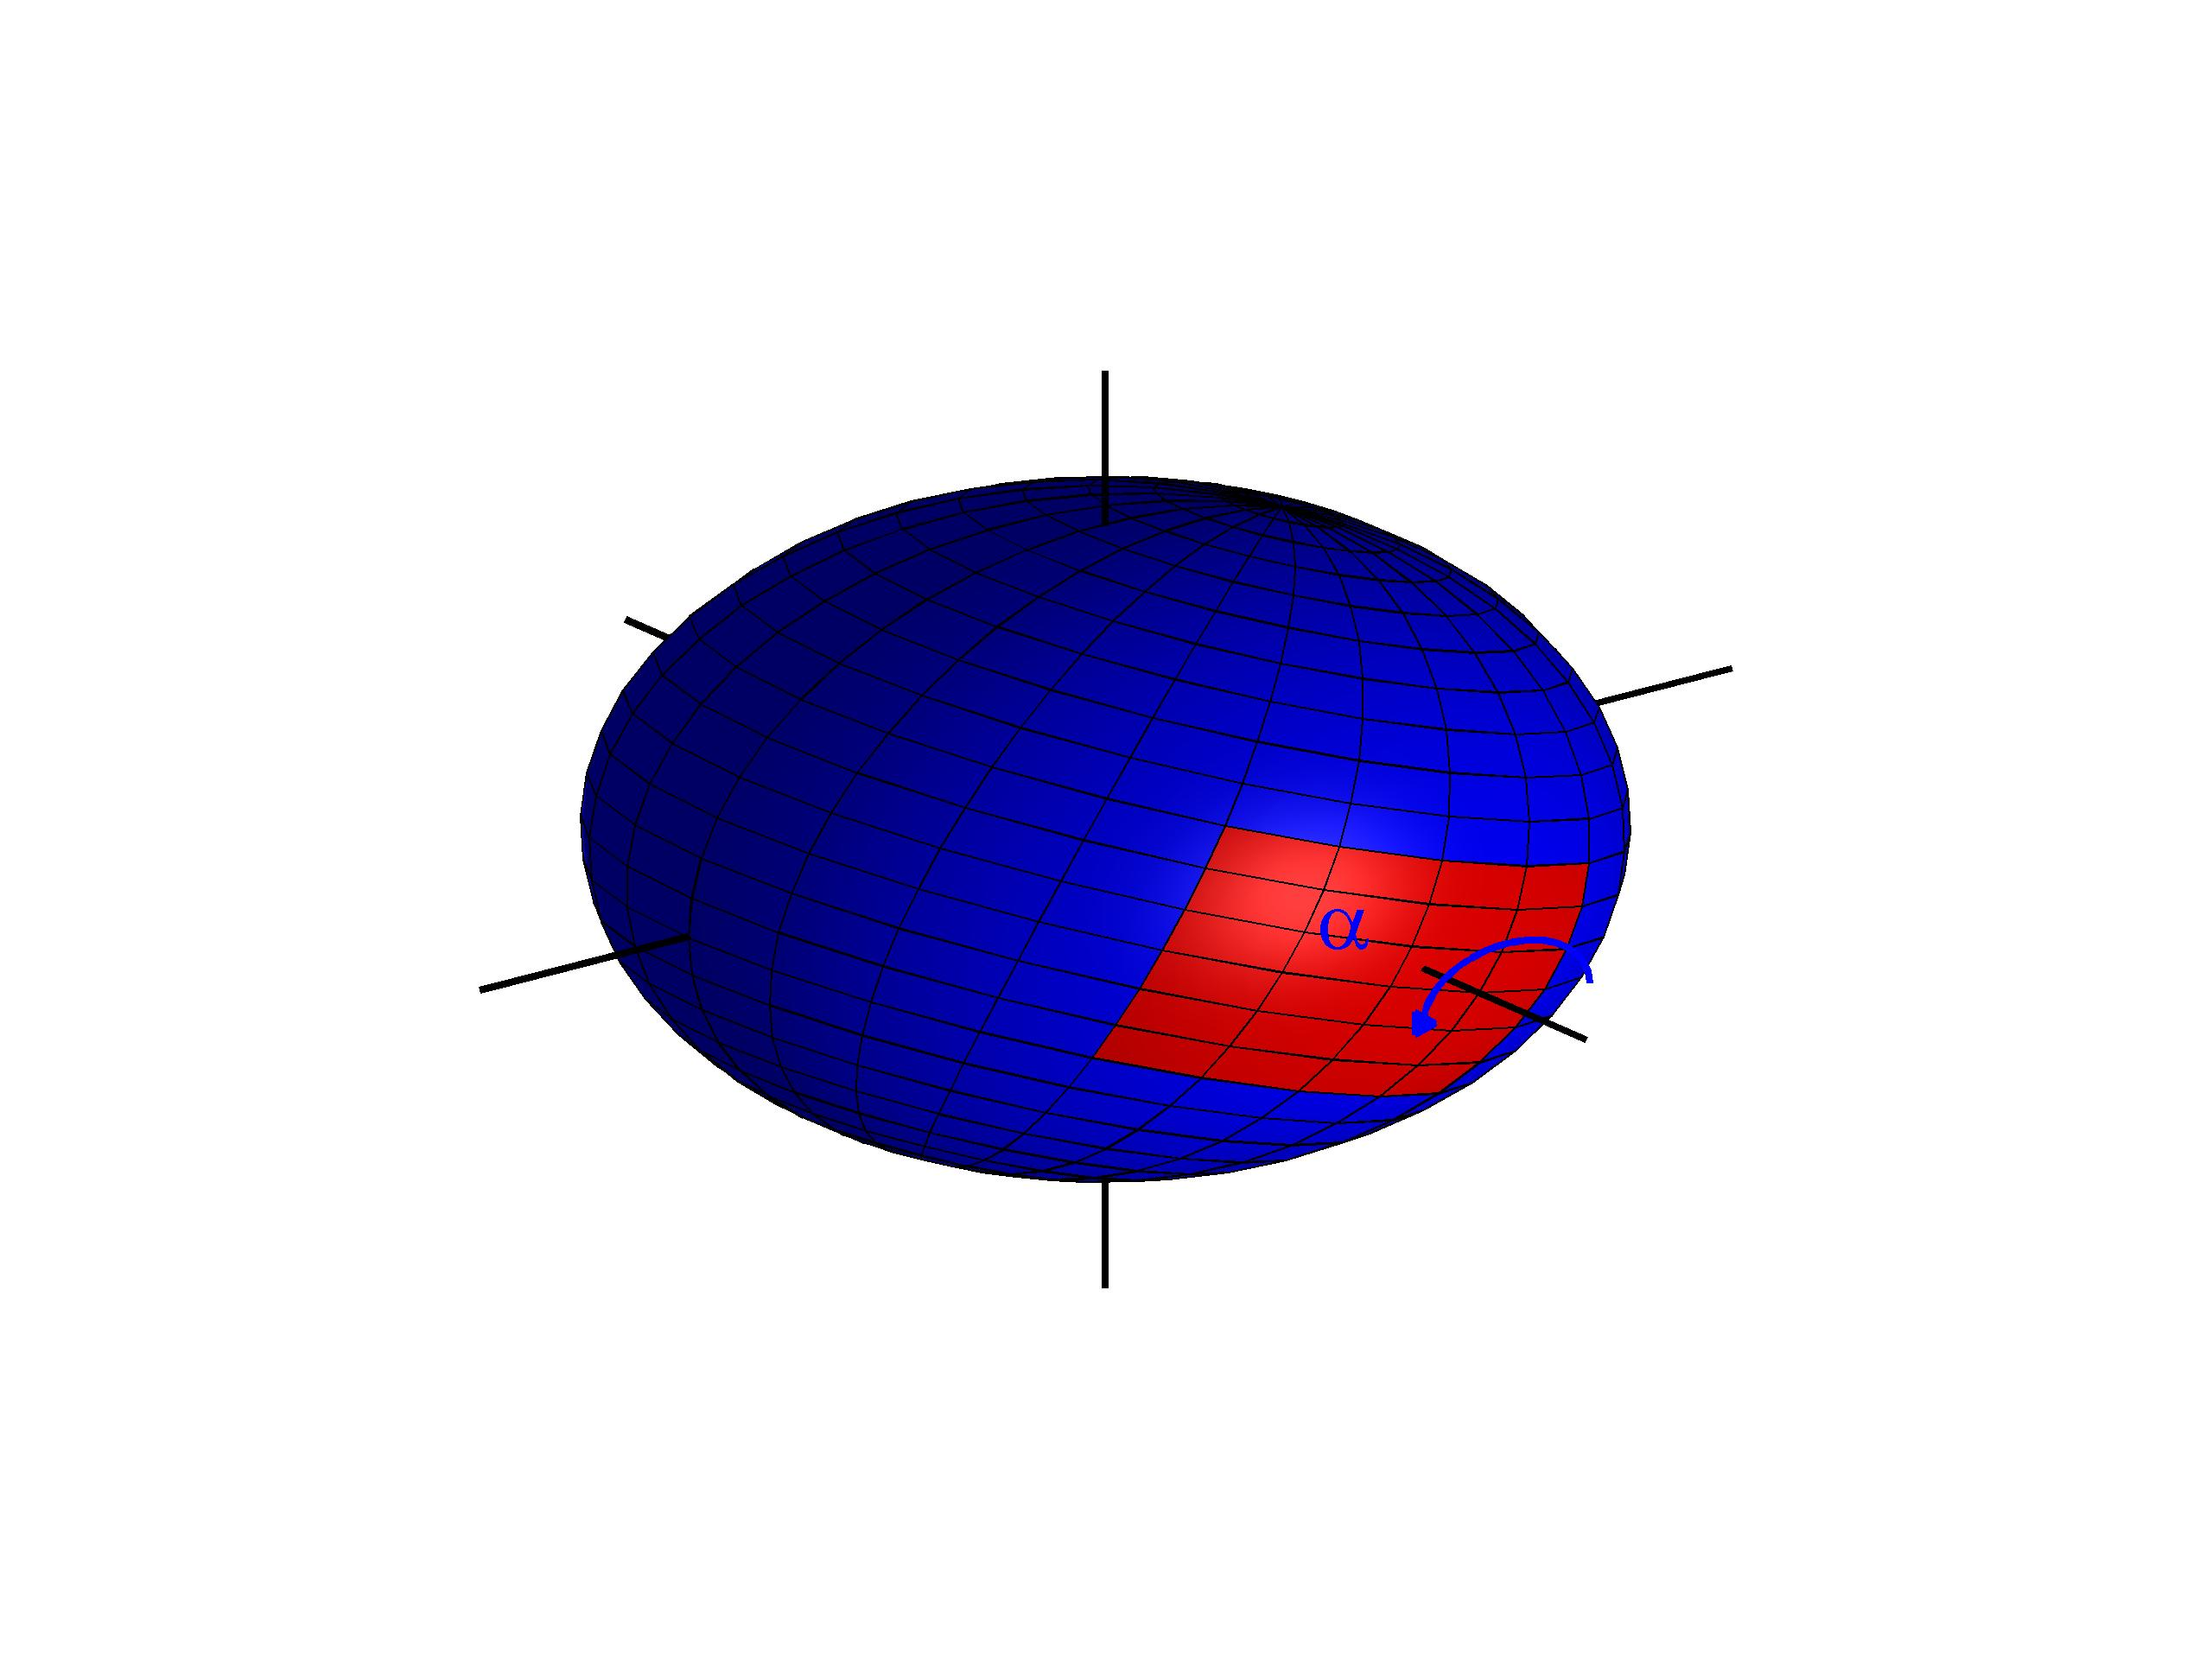
\includegraphics[width=\textwidth]{sphere_2}
%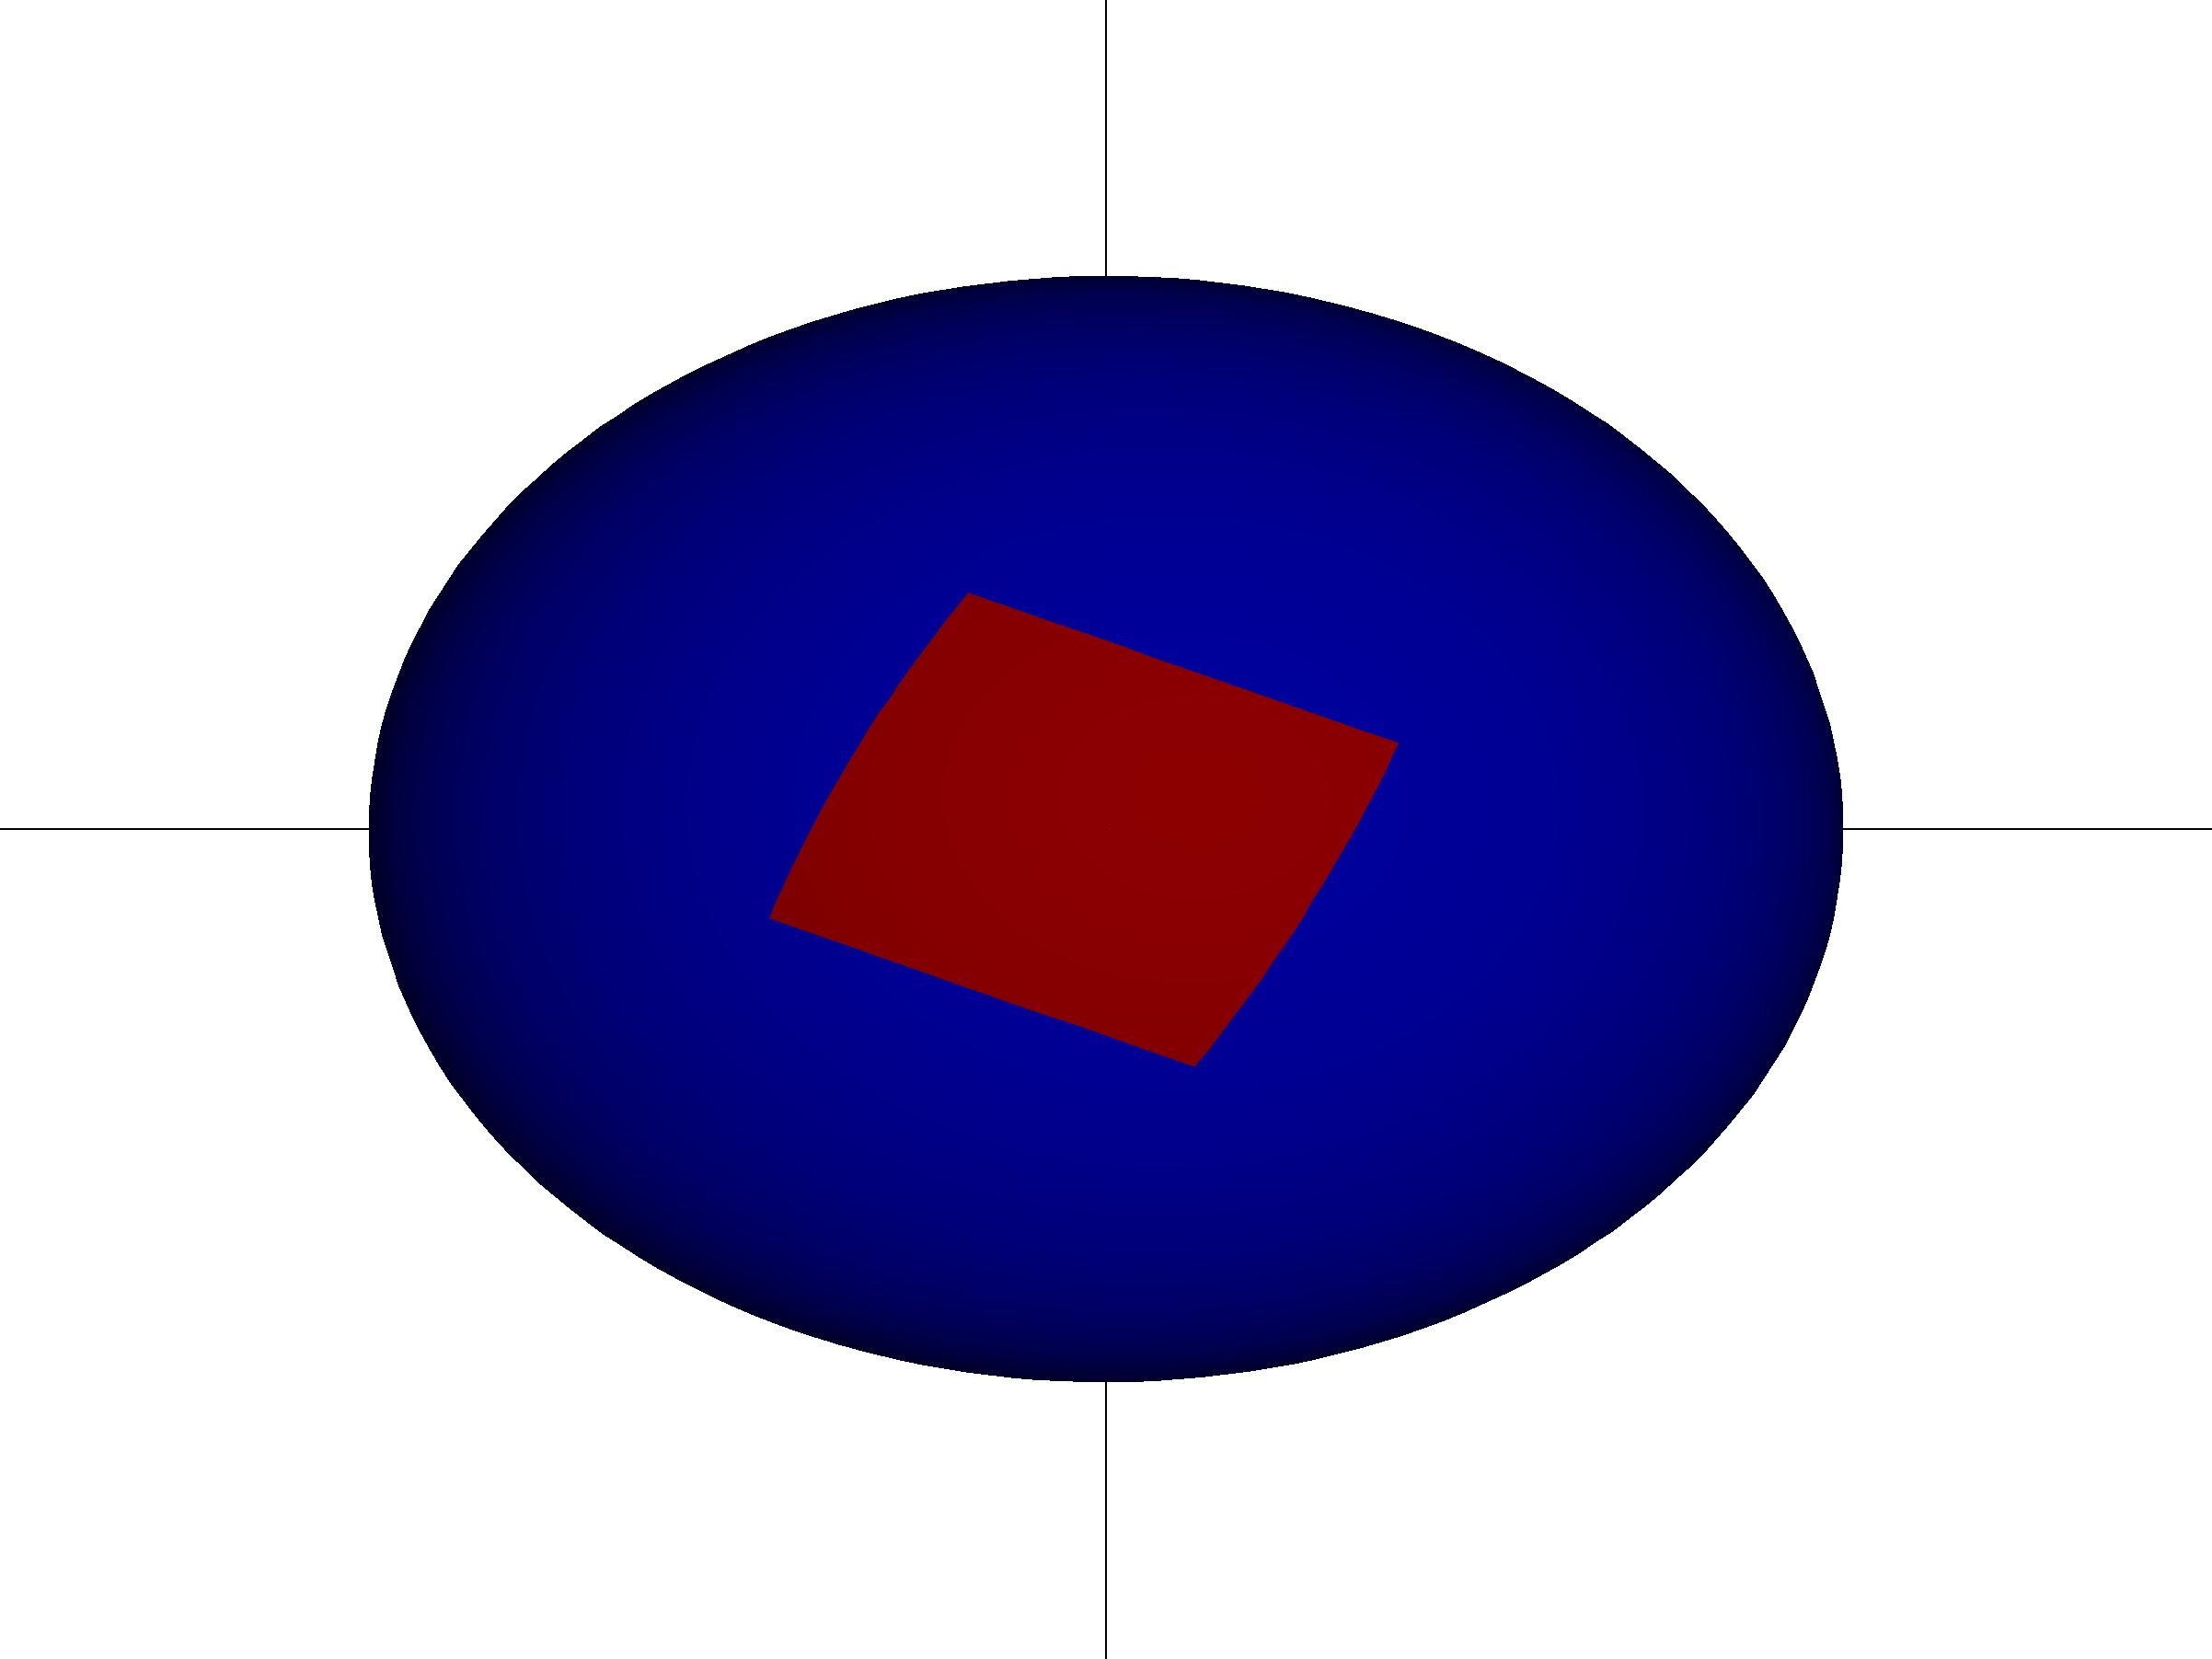
\includegraphics[width=\textwidth]{sphere2_2}
%\caption{}
%\end{subfigure}
%\begin{subfigure}{0.2\textwidth}
%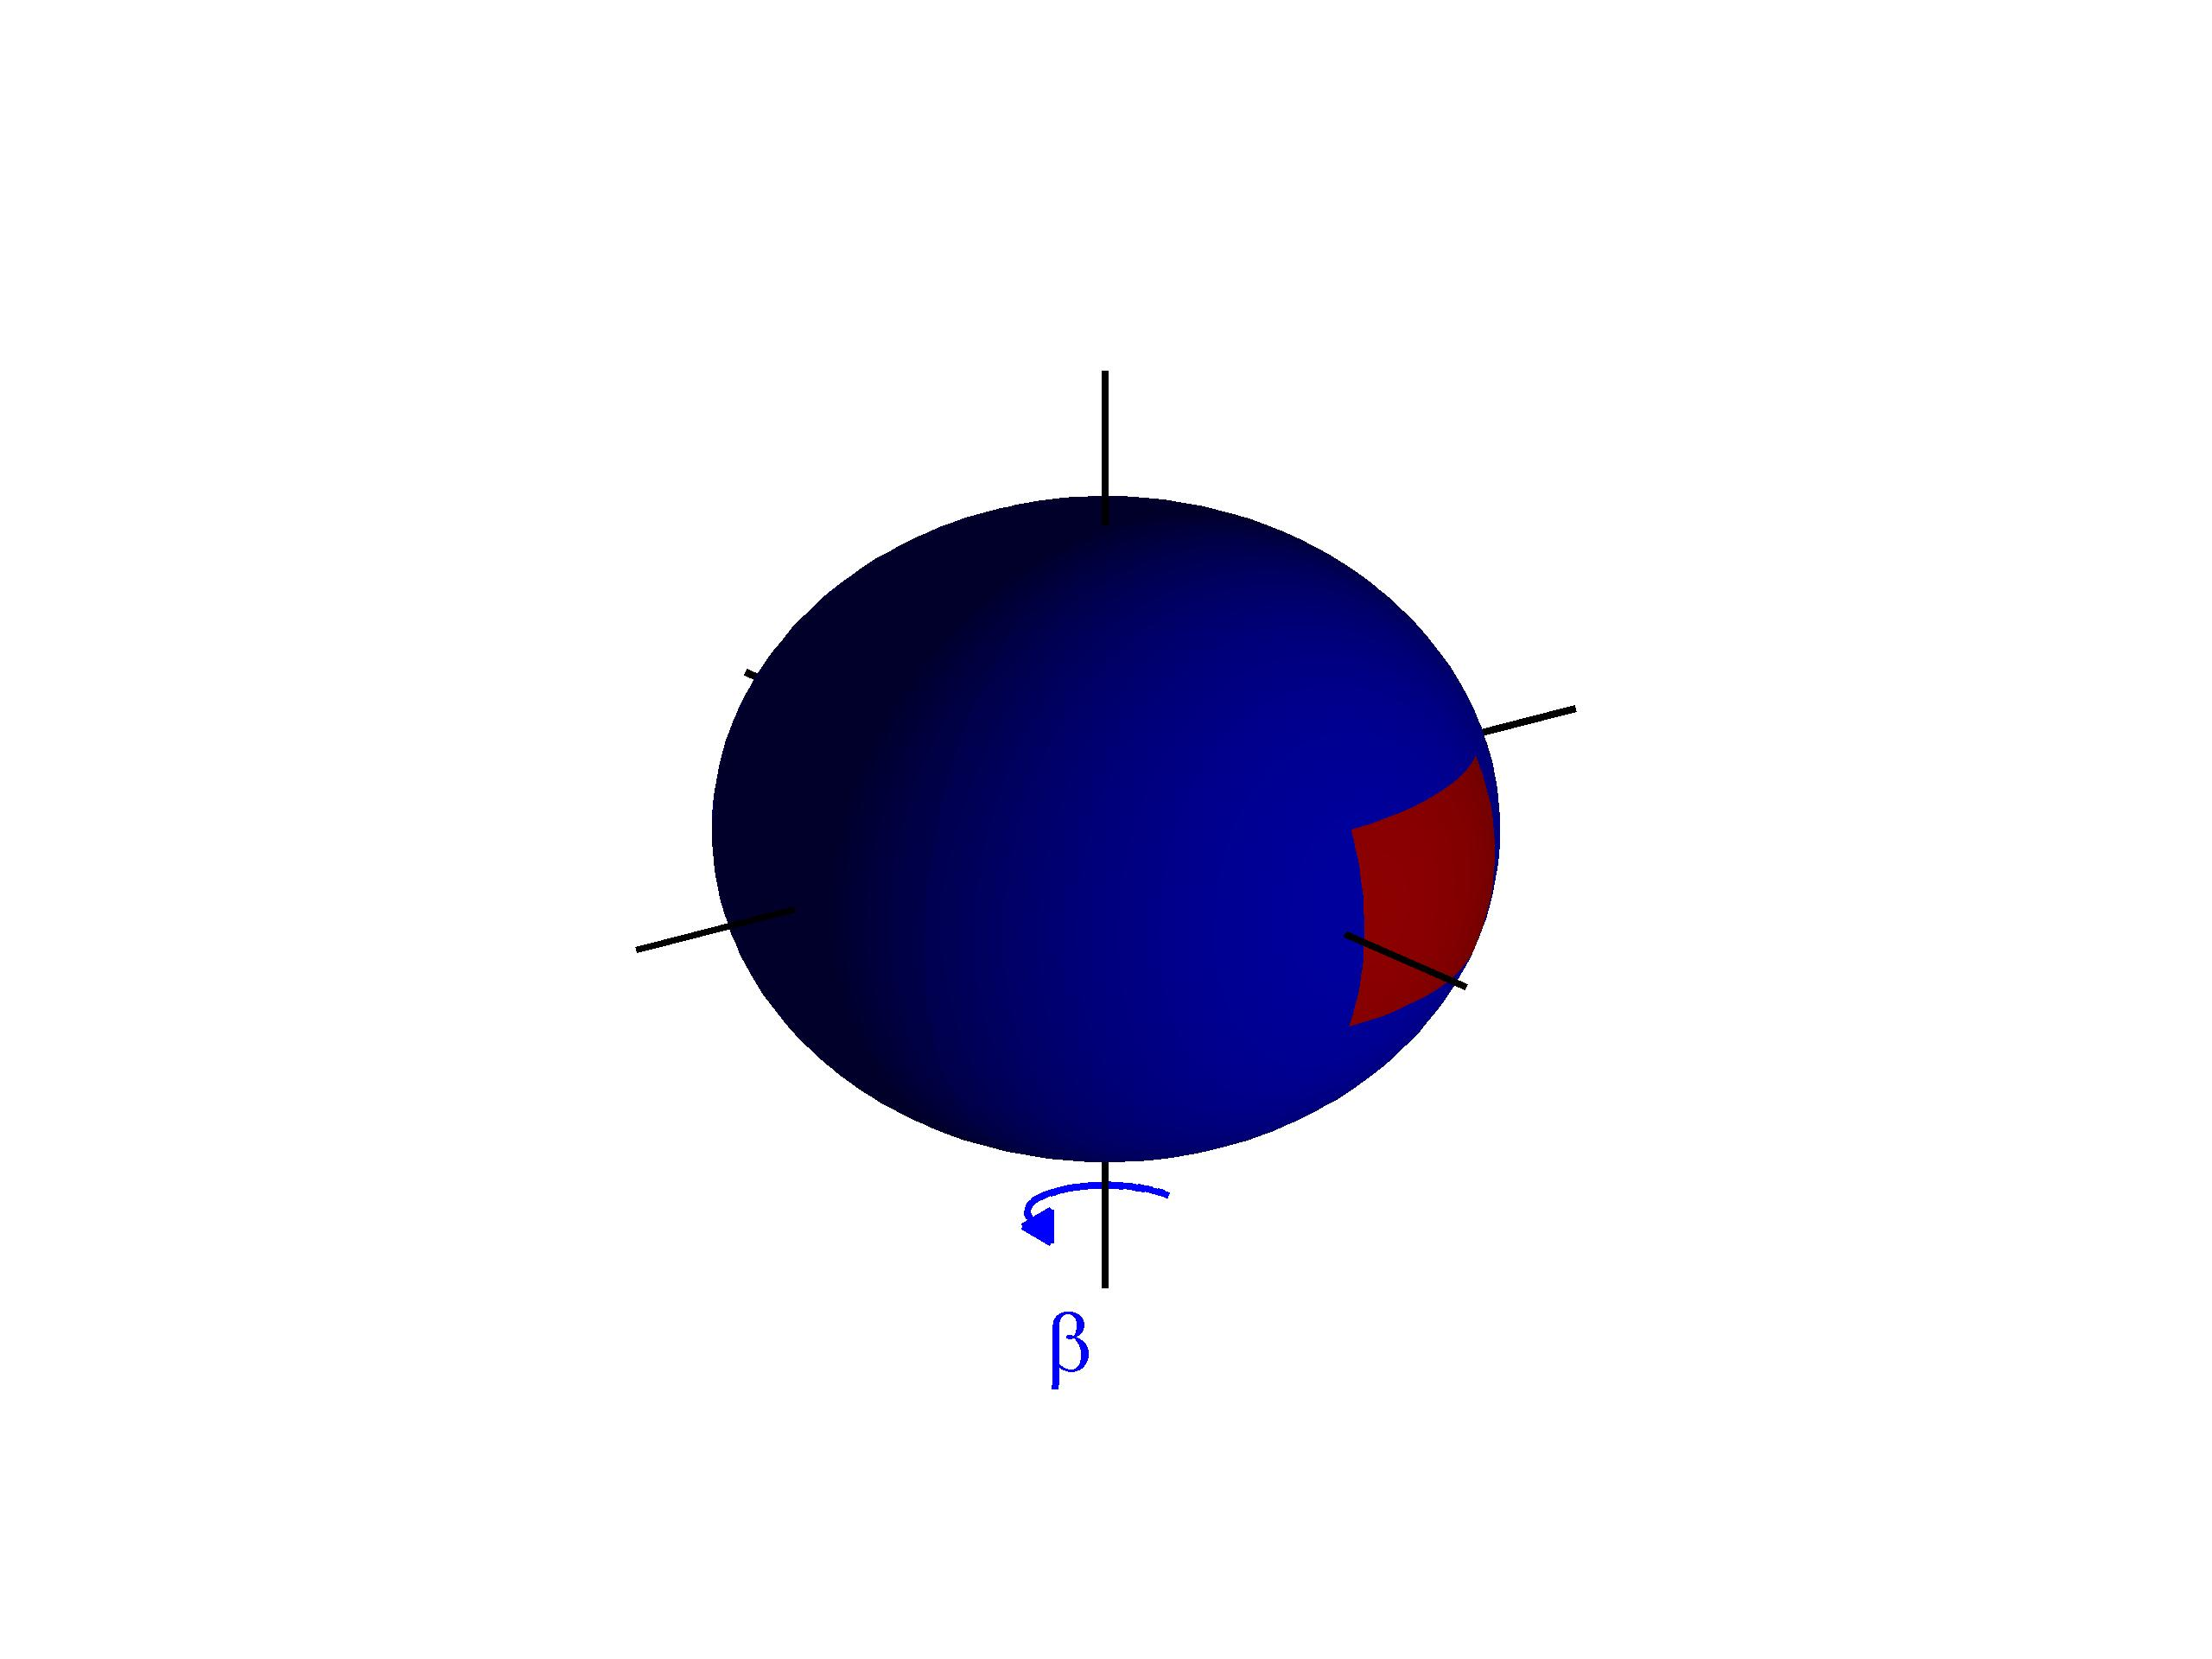
\includegraphics[width=\textwidth]{sphere_3}
%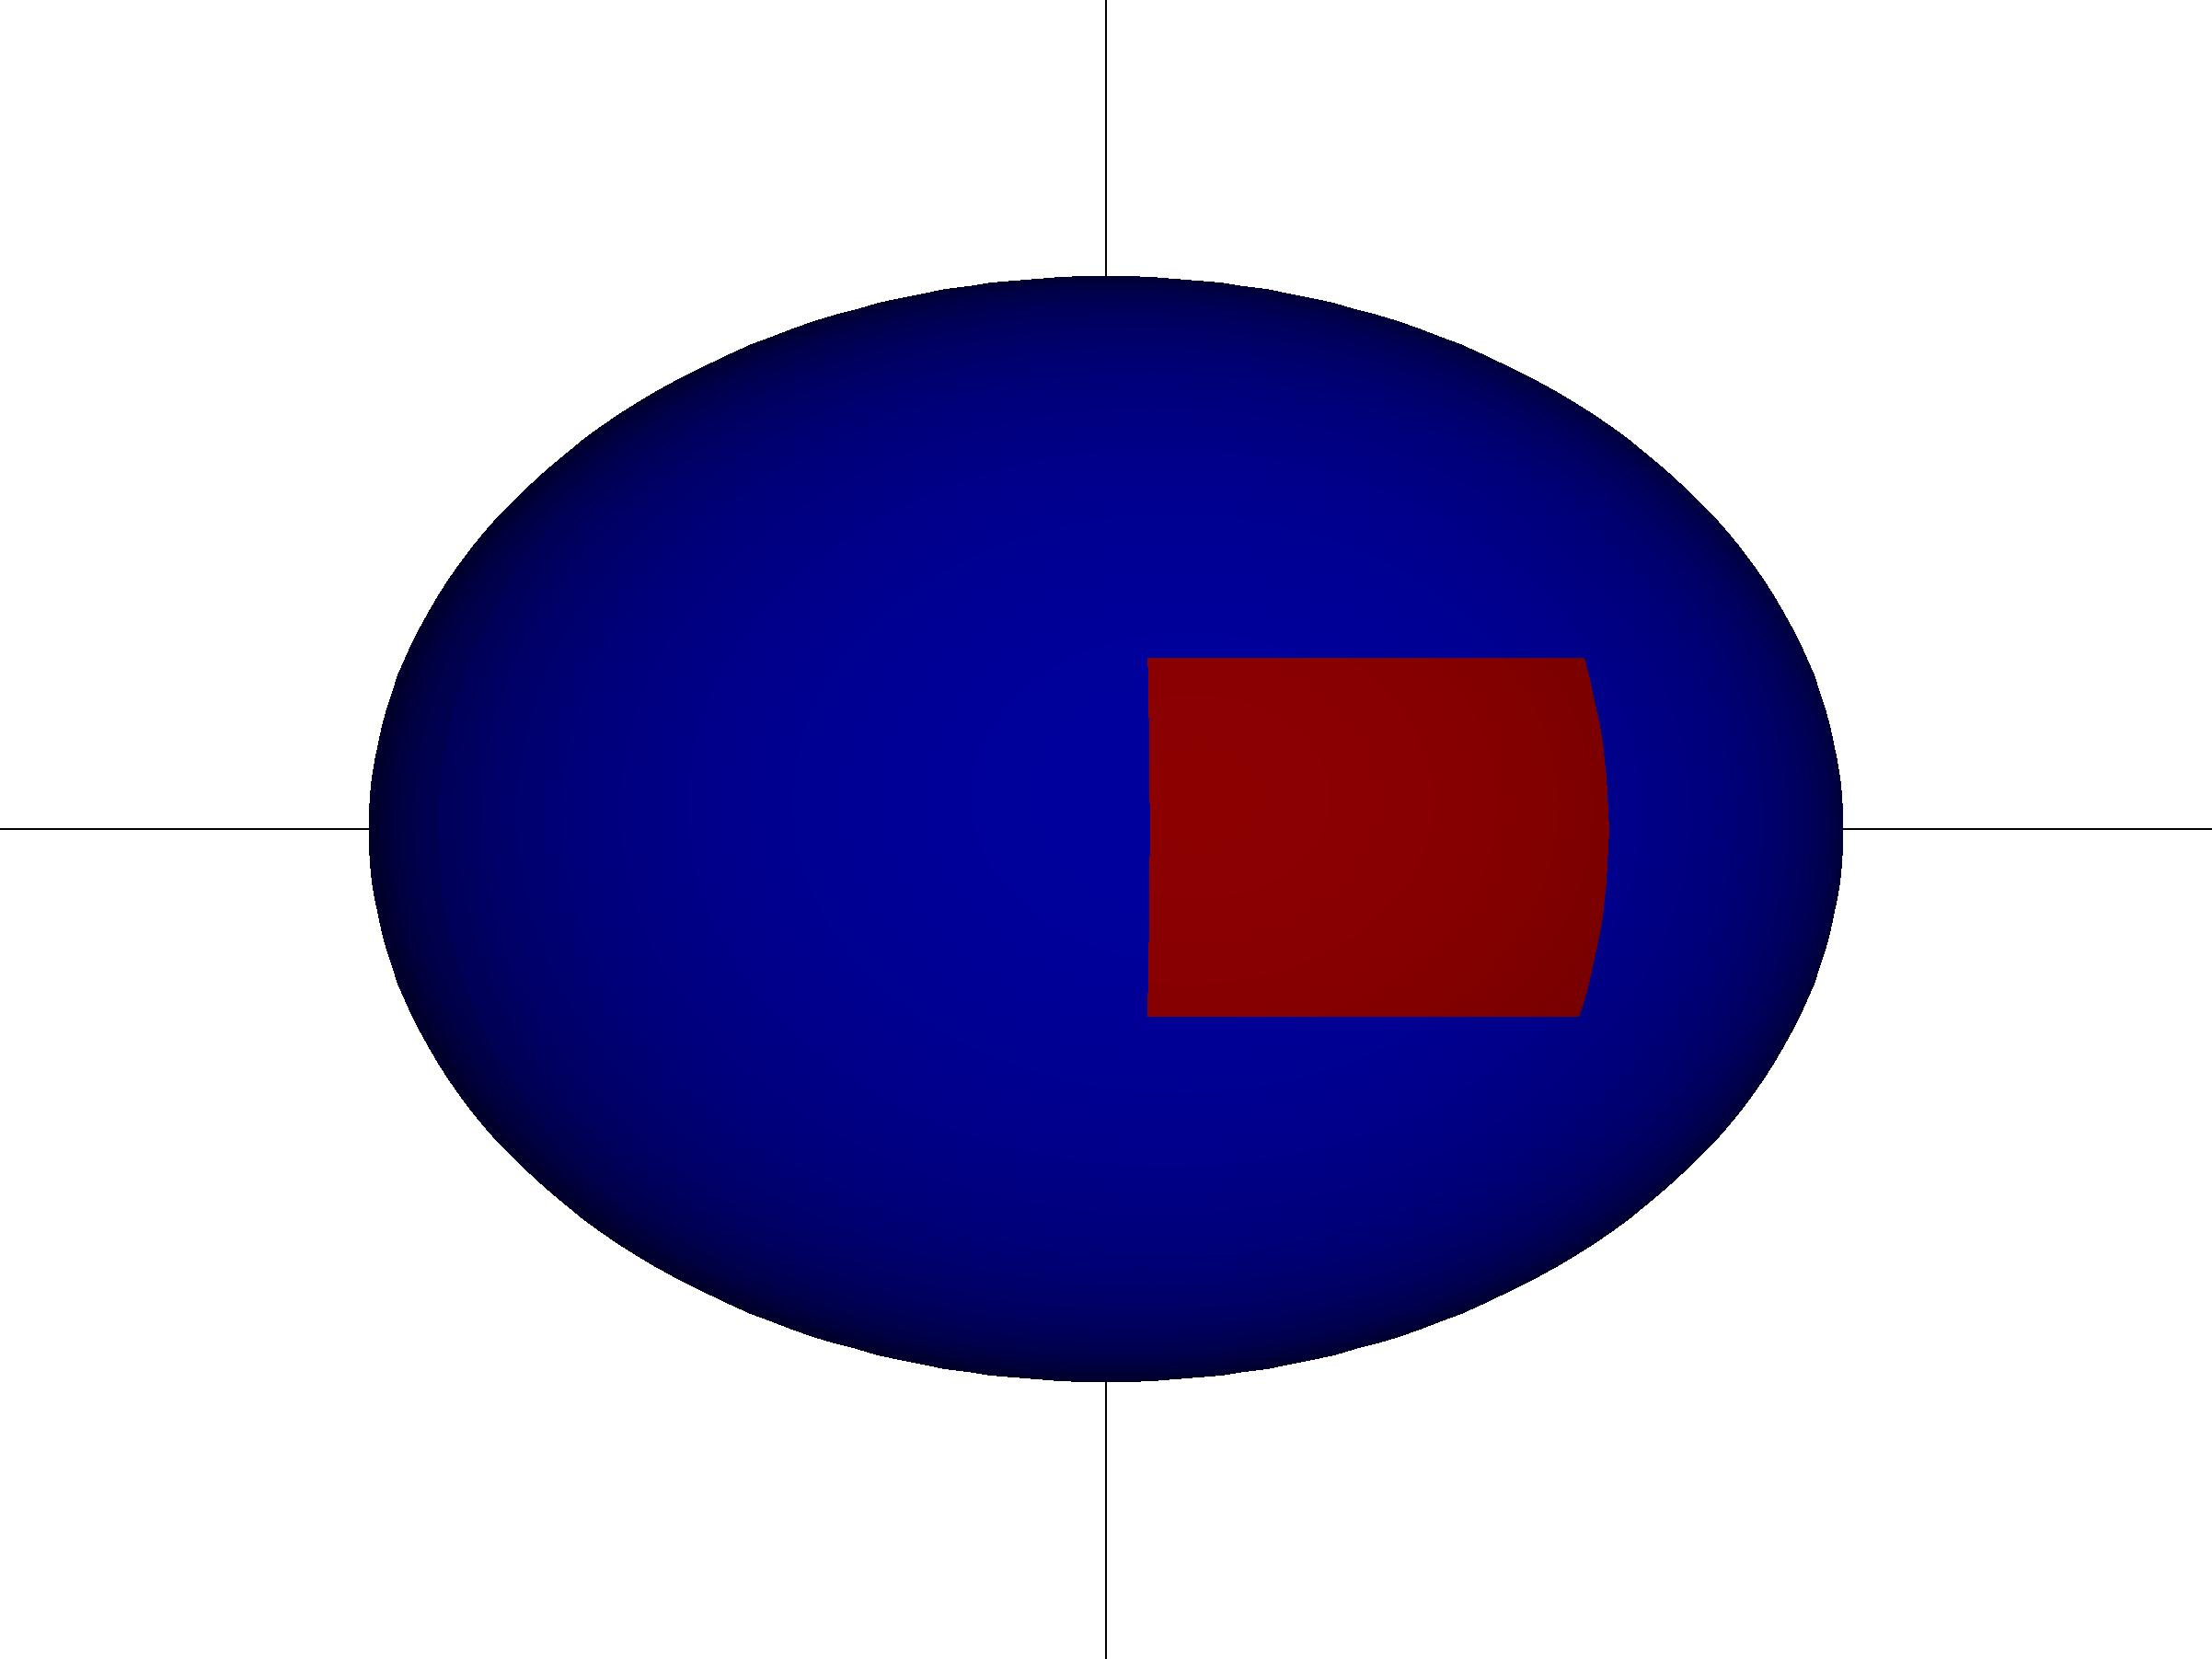
\includegraphics[width=\textwidth]{sphere2_3}
%\caption{}
%\end{subfigure}
%\begin{subfigure}{0.2\textwidth}
%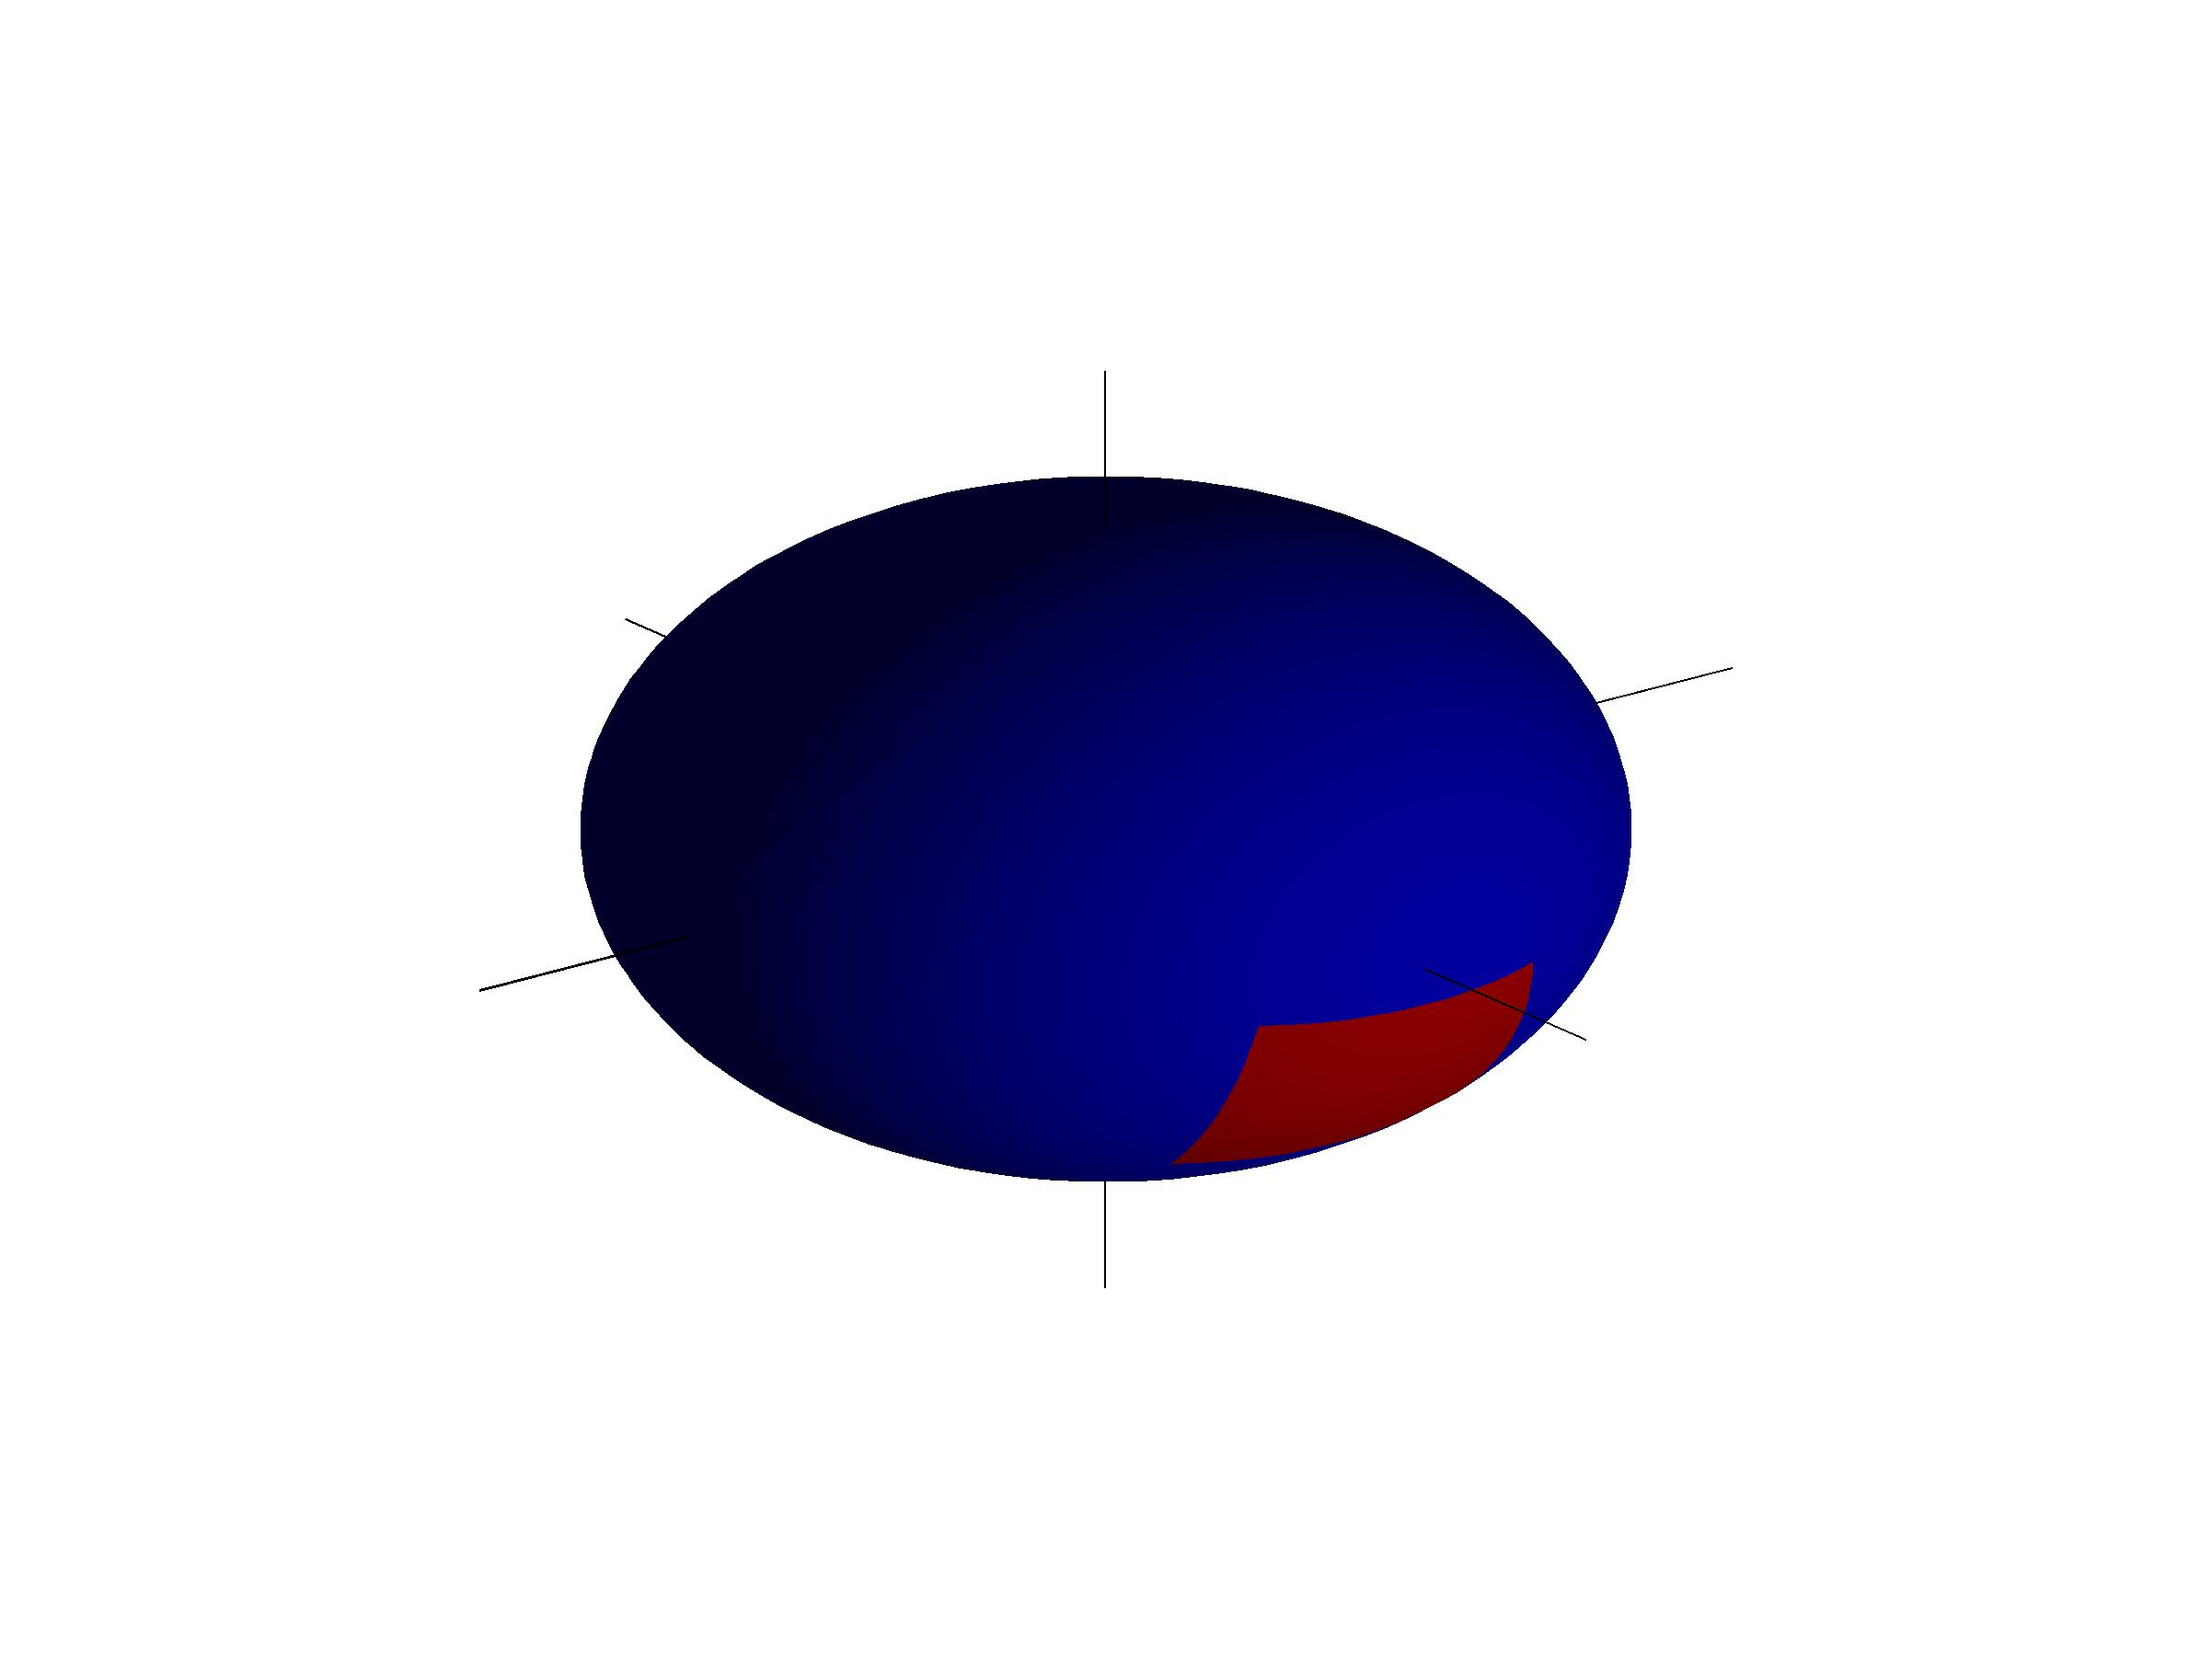
\includegraphics[width=\textwidth]{sphere_4}
%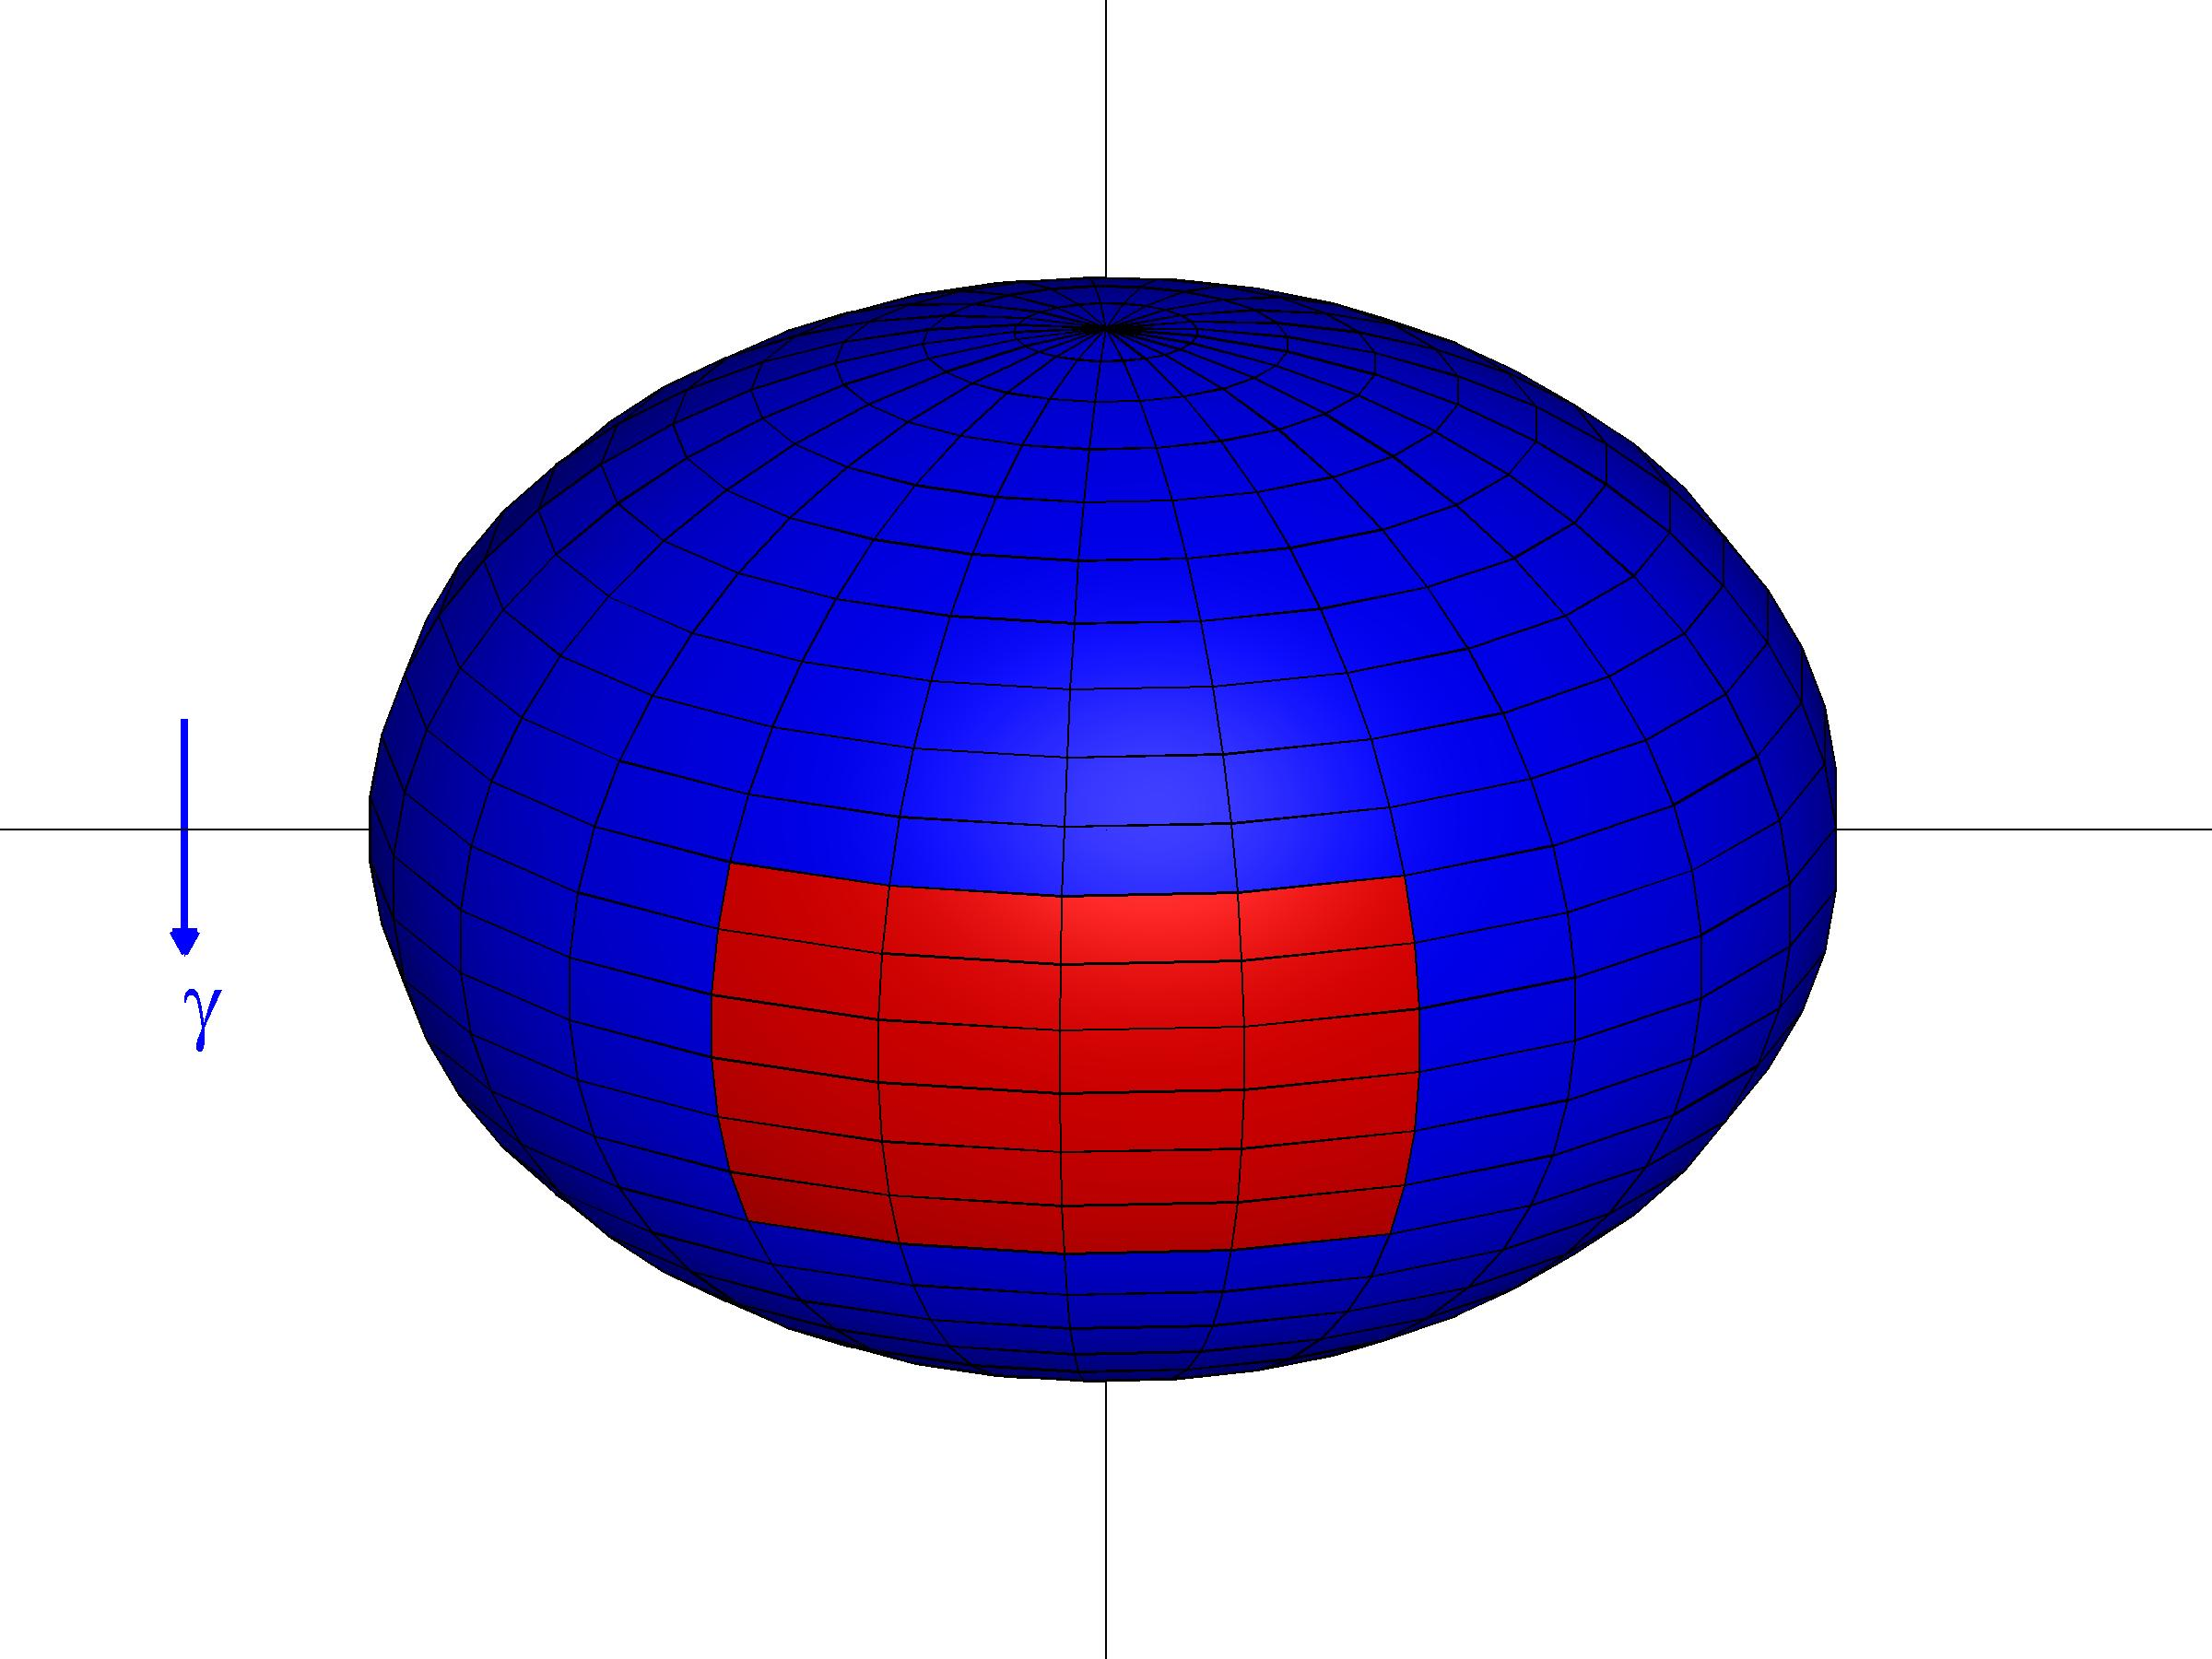
\includegraphics[width=\textwidth]{sphere2_4}
%\caption{}
%\end{subfigure}
%\caption{Illustration of how rotations in three dimensions correspond to translations and rotations in two dimensions. (a) The original image. (b) Rotation around the x-axis (Euler angle $\alpha$) in three dimensions corresponds to rotation of the image. (c) Rotation around the y-axis (Euler angle $\beta$) in three dimensions corresponds to horizontal translation. (d) Rotation around the z-axis (Euler angle $\gamma$) in three dimensions corresponds to vertical translation. The top row shows the three-dimensional spheres, and the bottom row shows the (two-dimensional) surface of the sphere in which we are interested.}
%\label{fig:SO3_picture}
%\end{figure*}

\end{document}

